\documentclass[6pt]{article}
\usepackage{amsmath}
\usepackage{graphicx}
\usepackage{caption}
\usepackage[landscape]{geometry}
\usepackage{multicol}
\usepackage{amssymb}
\usepackage{enumitem}
\usepackage{xcolor}
\usepackage{float}
\usepackage{geometry}
\usepackage{setspace} 
\definecolor{light-gray}{gray}{0.50}
 \geometry{
 a4paper,
 total={292mm,200mm},
 left=5mm,
 right=5mm,
 top=8mm,
 bottom=8mm
 }
\setcounter{section}{0}
\setlength\columnseprule{0.5pt}
\setlength{\parindent}{0pt}
\graphicspath{ {images/} }

\begin{document}
\begin{multicols*}{3}

%--------------------------------------------------------------
%MENGEN 
\subsection*{Mengen}
\begin{itemize}[itemsep=1pt, parsep=2pt, leftmargin=*,align=left]
	\item {\bf Teilmenge} (A $\subseteq$ B) \\ $x \in A \Rightarrow x \in B$
	\item {\bf Beschr{\"a}nkung} \\Es exisitieren $C_1$, $C_2$ sodass $\forall x \in M$ gilt: $C_1 \leq x \leq C_2$
	\item {\bf Obere/Untere Schranke} \\ Ist M nach oben beschr{\"a}nkt mit $C_2$, dann nennt alle $C \leq C_2$ eine obere Schranke (dito untere Schranke)
	\item {\bf Supremum} (sup A) = kleinste obere Schranke \\ 
				a = sup A, falls $\forall x \in A : x \leq a$ 
	\item {\bf Infimum} (inf A) = gr{\"o}sste untere Schranke	 \\  
				a = inf A, falls $\forall x \in A: x \geq a$ 
	\item {\bf Maximum / Minimum}	\\ muss immer zur Menge geh{\"o}ren \\
				 $inf M \in M \Rightarrow min M = inf M$ \\
				 $sup M \in M \Rightarrow max M = sup M$
\end{itemize}
Stetige Funktion auf einem kompakten Bereich nimmt stets ihr Min. und Max. an (Satz von Weierstrass )

% ---
\subsubsection*{Identit{\"a}ten / Tricks}
\begin{tabular}{lll}
$A \cup B = \lbrace{x | x \in A \land x \in B}\rbrace$ 
	& $A \cap B = \lbrace{x | x \in A \lor x \in B}\rbrace $ \\
$A^c =\lbrace{x | x \in A \land x \not\in B }\rbrace$ 
	& $A\backslash B = \lbrace{x | x \in A \lor x \in B}\rbrace$ \\
$sup(-A)  = - inf(A)$  
	& $inf(-A) = - sup(A)$	 \\
$max(-A) = -min(A)$
	& 	 $min(-A) = - max(A)$ \\
\end{tabular}
\vspace{8mm}
\begin{tabular}{lll}
$sup(A \cup B) = max\lbrace{sup A, sup B}\rbrace$ \\
$inf(A \cup B) = min\lbrace{inf A, inf B}\rbrace$  \\
Ist M abgeschlossen und beschr{\"a}nkt $\rightarrow \exists$ Min. und Max. \\
\end{tabular}

\vspace{-6mm}
\noindent\rule{9cm}{0.1pt}
\vspace{-5mm}

%--------------------------------------------------------------
%FUNKTIONEN 
\subsection*{Funktionen}
Sei f : X $\rightarrow$ Y eine Abbildung
\begin{itemize}[leftmargin=*,align=left]
	\setlength{\itemsep}{2pt}
		\item {\bf surjektiv}, falls jedes y $\in$ Y mind. ein Urbild hat. \newline
				 $\forall y \in Y \; \exists x \in X: y = f(x)$
		\item  {\bf injektiv}, falls jedes y $\in$ Y h{\"o}chstens ein Urbild hat. \newline
				 $ \forall x_1,x_2 \in X: f(x_1) = f(x_2) \implies x_1 = x_2$
		\item  {\bf bijektiv}, falls jedes y $\in$ Y genau ein Urbild hat. \newline
				 $\forall y \in Y \; \exists ! x \in X: y = f(x)$
		\item {\bf monoton steigend/fallend}, falls aus $x_1 < x_2$ immer $f(x_1) \leq f(x_2)$ folgt (respektiv $>$ $\rightarrow$ $\geq$)
		\item {\bf streng mononton steigend/fallend},  falls aus $x_1 < x_2$ immer $f(x_1) < f(x_2)$ folgt (respektiv $>$ $\rightarrow$ $>$)
	\end{itemize}
	
%\noindent\rule{9cm}{0.1pt}
\columnbreak


%--------------------------------------------------------------
%Komplexe Zahlen
\subsection*{Komplexe Zahlen}

\begin{tabular}{lll}
 Normalform 		&  z = x+iy \\
 Polarform 			&	$z = r (\cos \phi +i \sin \phi) = r \cdot e^{i \phi}$ \\ 
									& x =  $r \cos \phi$ \quad $y = r \sin \phi$ \\
 									&  $r = |z| =\sqrt{x^2+y^2}$ \\
 									& \\
 arg $\phi$ = arg(z) & $\left\{ \begin{array}{ll} + \arccos \tfrac{x}{|z|} & \text{falls } y \geq 0 \\ - \arccos \tfrac{x}{|z|} & \text{falls } y < 0 \\ \text{undef} & \text{falls } x = y = 0 \end{array} \right.$ \\
 									& \\
 				
(Tipps) 					& $i = e^{i \frac{\pi}{2}} $\quad $-i = e^{-i \frac{\pi}{2}} = e^{i 									\frac{3\pi}{2}}$ \\
 									&  $1 = -e^{i \pi} = e^{0}$ \quad $-1 = e^{i \pi} = i^2$ \\
 									& $z^{-1} = \frac{\overline z}{|z|^2} $ \\
 									& \\
 Konjugierte Form & $\overline z = x -iy = r \cdot e^{-i \phi}$\\				
 Realteil 				& $Re(z) = x = \frac{z+\overline z}{2}$  \\
Imagin{\"a}rteil 	& $Im(z) = y = \frac{z-\overline z}{2i}$\\
 \end{tabular}

% ---
\subsubsection*{Rechnen mit komplexen Zahlen}
\begin{onehalfspace} 
\begin{tabular}{lll}
Addi.			&   $z_1 \pm z_2 = (x_1 \pm x_2) + i(y_1 \pm y_2)$\\
Multipl. 		&  $z_1 \cdot z_2 = (x_1x_2 - y_1y_2) + i(x_1y_2 + x_2y_1)$\\
					&  $z_1 \cdot z_2 = (r_1 r_2) \cdot e^{i(\phi_1 + \phi_2)}$ \\
Potenz 			& $z^n = (r \cdot e^{i \phi})^n = r^n \cdot e^{in \phi}$ \\
Betrag 			& $ |z| = \sqrt{z \overline{z}} = \sqrt{x^2+y^2} = r$\\
Bruch 			& $\rightarrow$ mit komplex konjugiertem Nenner erweitern	\\
					& $\frac{3+4i}{4-3i} = \frac{(3+4i)*(4+3i)}{(4-3i)*(4+3i)} = \frac{12+9i + 16i -12 }{16+12i - 12i +9} = \frac{25i}{25} = i $ \\
					& \\
Wurzel 			& $\sqrt{\sqrt{3}i-1} \Rightarrow $ Substitution $\sqrt{u}$ mit u = $					\sqrt{3}i-1$  \\
					& (1) u in Polarkord. $|u|=\sqrt{\sqrt{3}^2 + 1^2}=2$ \\
					& $\phi = arccos(\frac{x}{|z|}) = arccos(\frac{-1}{|2|}) = \frac{2\pi}{3}$ \\
					& $\Longrightarrow  u=2e^{i\frac{2\pi}{3}}$ \\ 
					& (2) einsetzen in $\sqrt{u} \rightarrow \sqrt{2e^{i\frac{2\pi}{3}}} = \sqrt{2}e^{\frac{\pi}{3}} $ \\
					& (3) $x=rcos(\phi)$ , $y=rsin(\phi) \Rightarrow \sqrt{2}(\frac{1}{2}+i\frac{\sqrt{3}}{2})$
\end{tabular}
\end{onehalfspace} 
\vspace{-3mm}

% ---
\subsubsection*{Einheitswurzeln}
\begin{onehalfspace} 
\begin{tabular}{lll}
Moivre-Formel: & $z^n = r^ne^{n\phi i} = r^n(cos(n\phi)+ isin(n\phi))$  \\
n'te Wurzeln: 	&	$w_k = \sqrt[n]{r}(cos(\frac{\phi + 2k\pi}{n}) + isin(\frac{\phi + 2k							\pi}{n})$ \\ 
						& wobei k= 0,.., n-1\\
\end{tabular}
\end{onehalfspace} 

%\noindent\rule{9cm}{0.1pt}
%--------------------------------------------------------------
%FUNKTIONEN
\subsection*{Folgen}
Eine reele Folge heisst... 	
\vspace{3mm}\\
\begin{onehalfspace}
\begin{tabular}{lll}
konvergent: 				& wenn  $\lim\limits_{n \to \infty}  a_n$ existiert\\
divergent: 				&  wenn $\lim\limits_{n \to \infty}  a_n$  nicht existiert\\
Nullfolge: 					&  wenn $\lim\limits_{n \to \infty}  a_n$ = 0 ist\\
alternierend:				& wenn die Vorzeichen der Folgenglieder \\
								&	abwechseln\\
absolut konvergent: 	& wenn $\lim\limits_{n \to \infty} \mid a_n \mid$ existiert \\
unbeschr{\"a}nkt:		& falls $a_n$ nicht beschr{\"a}nkt ist \\
								& $\longrightarrow$ Solche Fkt. sind stets divergent \\
\end{tabular}
\end{onehalfspace}
\vspace{-2mm}

\subsubsection*{H{\"a}ufungspunkte}
Ein H{\"a}ufungspunkt ist ein Grenzwert (Limes) einer Teilfolge.
\begin{itemize}[itemsep=2pt, parsep=2pt]
	\item Limes superior = gr{\"o}sster H{\"a}ufungspunkt
	\item Limes inferior = kleinster H{\"a}ufungspunkt
\end{itemize}
\vspace{-6mm}

\begin{enumerate}[label=(\roman*), itemsep=2pt, parsep=2pt]
		\item $\lim\limits_{n \to \infty}  a_n$, so ist der Limes a einziger H{\"a}ufungspunkt der Folge $a_n$ und jede Teilfolge konvergiert auch gegen a. 
		\item $a_n$ zwei verschiedene H{\"a}ufungspunkte $\rightarrow$ Folge ist divergent
\end{enumerate}



\subsubsection*{Satz von Bolzano-Weierstrass}
Jede beschr{\"a}nkte Folge $a_n$ - d.h eine f{\"u}r die gilt $\exists M \; \forall n:\, |a_n|<M$ - besitzt eine 
		konvergente Teilfolge bzw. einen H{\"a}ufungspunkt. (Satz von Bolzano-Weierstrass) 
		
\subsubsection*{Monotone Konvergenz}
				Sei $a_n$ eine nach oben (unten) beschr{\"a}nkte Folge und monoton wachsend (fallend). 	Dann konvergiert $a_n$ mit 
					
					\begin{equation*}
  							\lim_{n \to \infty} a_n = \sup_{n \in \mathbb{N}} a_n \quad \text{bzw.} \quad  \lim_{n \to \infty} a_n = \inf_{n \in\mathbb{N}} a_n
					\end{equation*}


\columnbreak

\subsubsection*{Cauchy-Folge}
Folge bei welcher der Abstand zwischen den Folgeglieder im Verlauf der Folge beliebig klein wird. 
\vspace{0mm}\\
\begin{equation*}
	\forall \epsilon>0 \; \exists n_0 = n_0(\epsilon) \in \mathbb{N} \; \forall n,l \geq n_0: | a_n - a_l | < \epsilon	
\end{equation*}

\begin{center}
	\framebox[1\width]{ Jede Cauchy-Folge $\longleftrightarrow$ konvergente Folge (im $\mathbb{R}^n$)  } \par
	\vspace{5mm}
	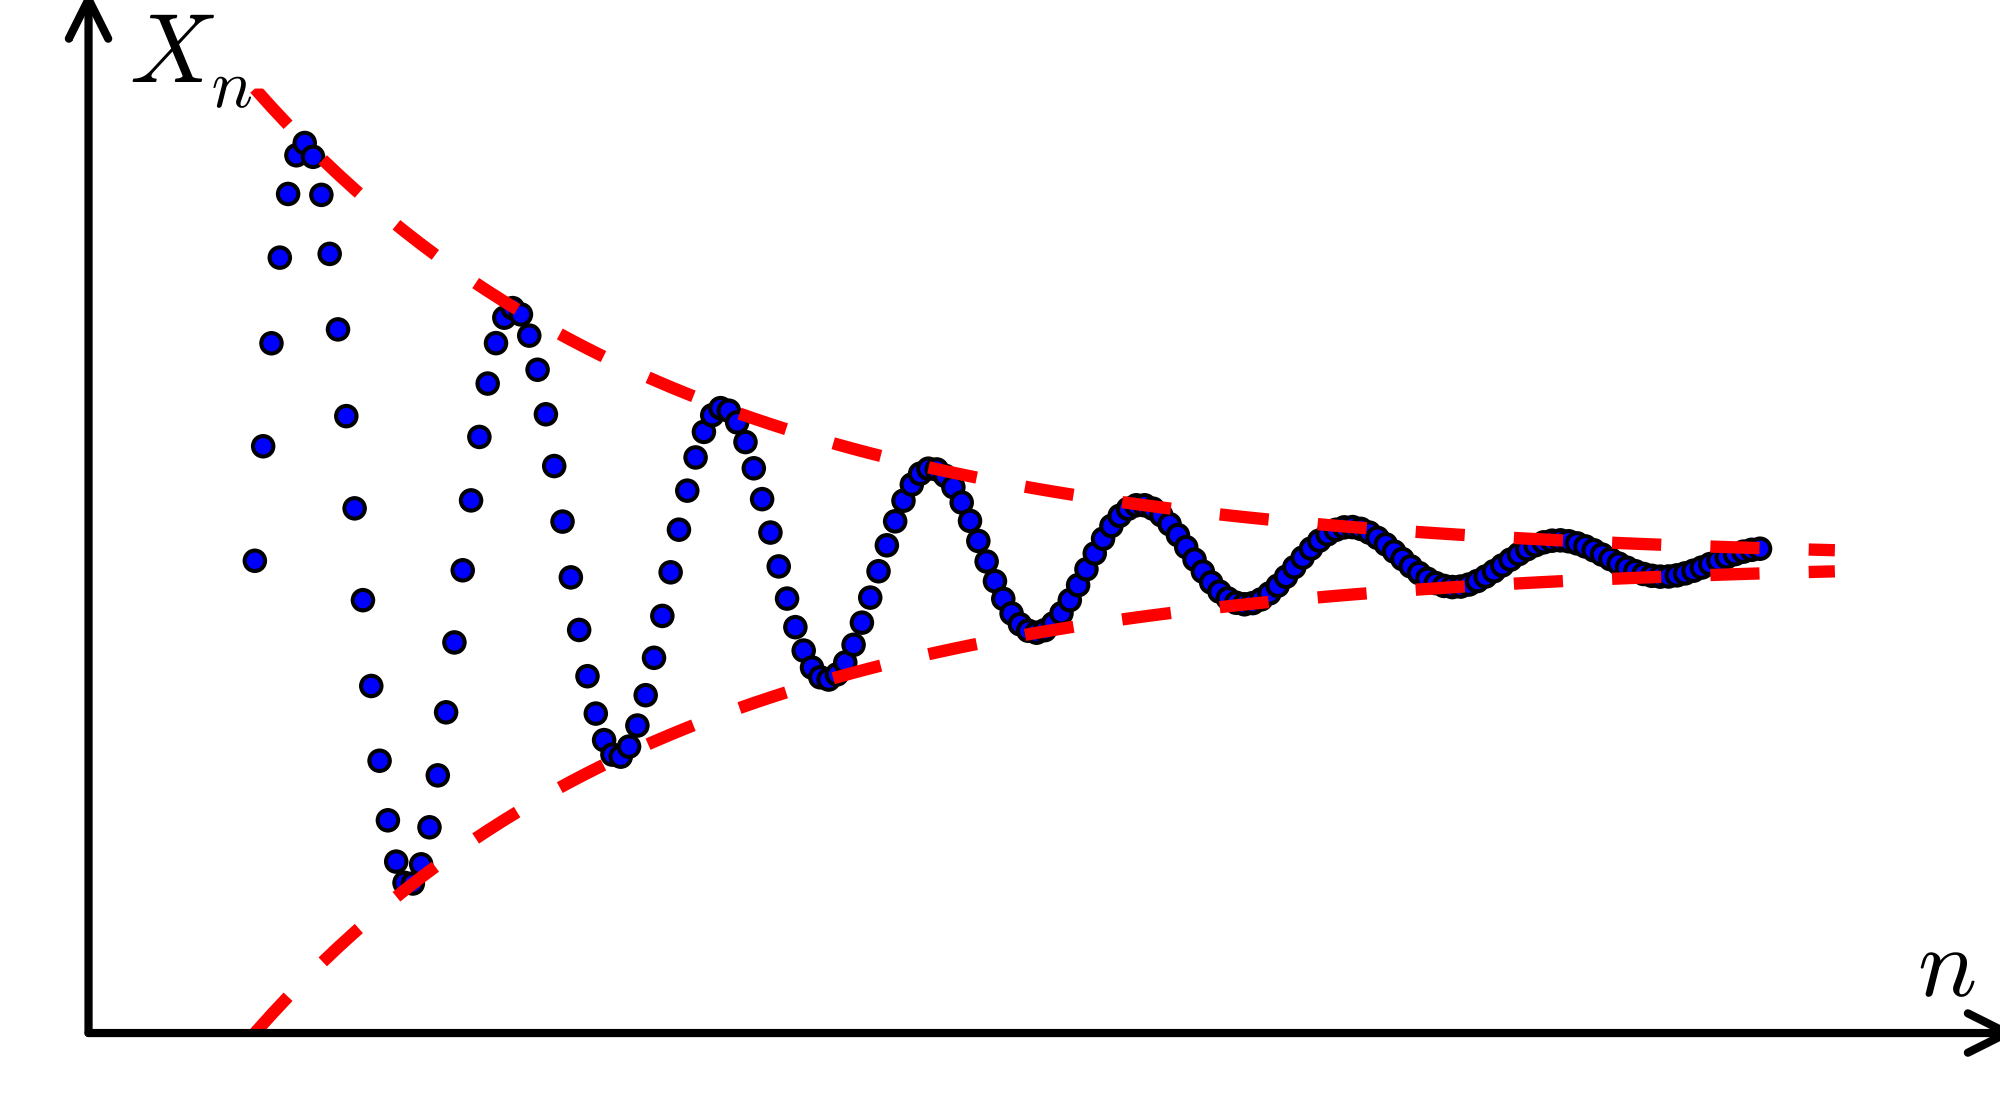
\includegraphics[width=150pt]{images/cauchy_folge}
\end{center}



\subsubsection*{Grenzwerte Regeln}
Sei $\lim\limits_{n \to \infty}  a_n=a$ und $\lim\limits_{n \to \infty} b_n=b$, dann gilt: \newline
\vspace{-5mm}
\begin{enumerate}[label=(\roman*)]
	\item $\lim\limits_{n \to \infty}  a_n + b_n=a + b$ 
	\item $\lim\limits_{n \to \infty}  a_n * b_n=a * b$
	\item $\lim\limits_{n \to \infty}  k * a_n= k * a$
	\item $\lim\limits_{n \to \infty}  \frac{a_n}{b_n}= \frac{a}{b}$, falls b$\not=$ 0
	\item Falls $a_n \leq b_n \implies a \leq b$
\end{enumerate}
\vspace{0mm}

	\subsubsection*{Verfahren / Tricks (zur Grenzwertbestimmung)}   

	\underline{Dominanz}  \\
	$x \to +\infty \quad... < \log(\log(x)) < \log(x) < x^\alpha < \alpha^x < x! < x^x$ \\
	$x \to 0 \quad \>\>\>\>\>\>... < \log(\log(x)) < \log(x) < (\frac{1}{x})^\alpha$ \\

	% Brüche Verfahren	
   \underline{Br{\"u}che}  \\
   			$\rightarrow$ durch st{\"a}rksten-wachsenden Term des Nenners dividieren 
   			\begin{equation*}
  					\lim\limits_{n \to \infty} \frac{n^2 + ln(n)}{\sqrt{n^4-n^3}} = 
  					\lim\limits_{n \to \infty} \frac{n^2 + ln(n)}{n^2 \sqrt{1- \frac{1}{n}}} =
  					\lim\limits_{n \to \infty} \frac{1 + \frac{ln(n)}{n^2}}{\sqrt{1- \frac{1}{n}}} 
					\rightarrow 1
			\end{equation*} \vspace{1mm}
		\vspace{-2mm}
  			\noindent\textcolor{gray}{\rule{9cm}{0.1pt}}
		\vspace{-2mm}\\
		
			
			
	% Wurzeln Verfahren			
   \underline{Wurzeln} \\
   \vspace{-4mm}
  	\begin{equation*}
  						\lim_{x\to\infty} \sqrt{\alpha}+\beta = \lim_{x\to\infty}(\sqrt{\alpha}+\beta)\frac{\sqrt{\alpha}-\beta}{\sqrt{\alpha}-\beta}	
  	\end{equation*}
%  	 \vspace{-2mm}
%  	\noindent\textcolor{gray}{\rule{9cm}{0.1pt}}
%	\vspace{-2mm}\\
  	
  	% l'hopital Verfahren				
   \underline{Bernoulli-de-l'hopital} \hspace{10mm} $\frac{0}{0}$ , $\frac{\infty}{\infty}$ , $0*\infty$ , $\infty - \infty$ \\
     \begin{onehalfspace} 
		\begin{tabular}{lll}	
		    \vspace{-3mm} \\
			F{\"u}r $\frac{0}{0}$ / $\frac{\infty}{\infty}$ : 	& $\lim\limits_{x \to a} \frac{f(x)}{g(x)} =\lim\limits_{x \to a} \frac{f'(x)}																															{g'(x)} $ \\
																						\vspace{0mm} \\
			F{\"u}r $0*\infty$ :											&  $\lim\limits_{x \to a} f(x) * g(x) = \lim\limits_{x \to a} \frac{f(x)}{\frac{1}																														{g(x)}}$ \\
																					& $ \rightarrow$  Typ  $\frac{0}{0}$ oder $\frac{\infty}{\infty} \longrightarrow$ l'Hopital anwenden \\
																					 	\vspace{-1mm} \\
		F{\"u}r $\infty -\infty$:											& $\lim\limits_{x \to a}\frac{f(x)}{g(x)} - \frac{h(x)}{j(x)} = \lim\limits_{x \to a} \frac{f(x)i(x)-h(x)g(x)}																					{g(x)i(x)}$
																						\vspace{3mm} \\
		\end{tabular}
	\end{onehalfspace}
	\vspace{-2mm}
	\noindent\textcolor{gray}{\rule{9cm}{0.1pt}}
	\vspace{-5mm} \\

   
   	% Potenz Trick	  
  	 \underline{$e^{log(x)}$ Trick} \hspace{28mm} $0^{0}$ , $\infty^0$ , $1^{\infty}$ \\
   		\begin{onehalfspace} 
			\begin{tabular}{lll}
			 		\vspace{-3mm} \\
					(i) Funktion umschreiben:  $f(x)^{g(x)} = e^{g(x)log(f(x))}$ 	\\
					(ii) L'Hopital anwenden im Exponenten \\
					 (da $e^x$: $\mathbb{R} \longrightarrow \mathbb{R}_+$  stetig ist, d{\"u}rfen wir den Limes in den \\
					 Exponenten ziehen )
					 \vspace{3mm} \\
			\end{tabular}
		\end{onehalfspace}
   		\vspace{-2mm} 
  		\noindent\textcolor{gray}{\rule{9cm}{0.1pt}}
		\vspace{-5mm}\\


	%Einschliessungskriterium (Satz der 2 Polizisten)
   \underline{Sandwich}\hspace{5mm} $g(x) \leq f(x) \leq h(x) $ mit  $\lim\limits_{x \to a}  g(x) = \lim\limits_{x \to a}  h(x) \\
   			\vspace{3mm}$\\
   			\begin{onehalfspace} 
				\begin{tabular}{lll}
			 			\vspace{-8mm} \\
			 			(i) Term in f(x) absch{\"a}tzen \\
			 			(ii) Grenzwerte von g(x) und h(x) bestimmen \\
			 			Falls nun $\lim\limits_{x \to a} g(x) = \lim\limits_{x \to a} h(x) = L$ gilt, $\longrightarrow \lim\limits_{x \to a} f(x) = L$
			 			\vspace{3mm} \\
			 			\underline{Bsp}: $\lim\limits_{x \to 0} x^2 sin(\frac{1}{x})$ \hspace{6mm}  $\rightarrow $ (i) $-1 \leq sin(\frac{1}{x}) \leq 1$ \\
			 			$g(x) = -x^2, h(x) = x^2 \>\> \rightarrow (ii) \lim\limits_{x \to 0} g(x) = \lim\limits_{x \to 0} h(x) = 0$ \\
			 			Folg. Sandwich-Theorem: $\lim\limits_{x \to 0} f(x) = 0$
			 			\vspace{3mm} \\
				\end{tabular}
			\end{onehalfspace}
 			\vspace{-2mm} 
 			\noindent\textcolor{gray}{\rule{9cm}{0.1pt}}
			\vspace{-6mm}\\
   	
   	
   	% Taylor Trick		
    \underline{Taylor}\hspace{35mm} (bei Schwierigen) \\
    	\vspace{-2mm} \\
   		Oft lassen sich schwierige Grenzwerte schneller mithilfe einer oder mehrer Taylorentwicklungen bestimmen.
   		$\rightarrow$ Dazu approximiert man einfach die Terme mithilfe Taylor! Es werden allerdings nur so viele Terme betrachtet bis sie sich gegenseitig nicht mehr aufheben.
		\vspace{4mm} \\
		N{\"u}tzliche Taylorentwicklungen: (an $x=0$)\\
			\begin{onehalfspace} 
				\begin{tabular}{lll}
						$e^x$ 			& =	& 	$1 + x  + \frac{x^2}{2} + \frac{x^3}{3!} +  \frac{x^4}{4!} + ...$ \\
						 $sin(x)$ 		& =	&	$x - \frac{x^3}{6} + \frac{x^5}{5!} + ... $ \\
						 $cos(x)$ 		& = 	& 	$1 + \frac{x^3}{6} + \frac{x^5}{5!} + ...$ \\
						 $log(1+x)$	& =	&  $x - \frac{x^2}{2} + \frac{x^3}{3} + ...$ \\
						 \vspace{-2mm}\\
				\end{tabular}
			\end{onehalfspace}
%			\vspace{-2mm}
%			\noindent\textcolor{gray}{\rule{9cm}{0.1pt}}
%			\vspace{-2mm}
		
	% Fundamental Limes
   \underline{Fundamental Limes}\\
   \vspace{-5mm}
   	\begin{equation*}
		\begin{split}
			\lim_{x \to a} \frac{\sin \odot}{\odot} = \lim_{x \to a} \frac{\tan \odot}{\odot} & = 1\ \text{mit}\ \odot \xrightarrow{\: x \to a \: } 0 \\ 
			\lim_{x \to a} (1 + \frac{1}{\odot})^\odot & = e\ \text{mit}\ \odot \xrightarrow{\: x \to a \: } \infty \\ 
			\lim_{x \to a} (1 + \odot)^\frac{1}{\odot} & = e\ \text{mit}\ \odot \xrightarrow{\: x \to a \: } 0 \\ 
		\end{split}
	\end{equation*}
	\vspace{-4mm}\\
   
   % Substitution
   \underline{Substitution}\\
   \vspace{-4mm}\\
   !! Eventuell Limes anpassen bei Substitution (siehe Beispiel)
   \vspace{-12mm}
   
   \begin{equation*}
   		\begin{split}
   			\lim\limits_{x \to \infty} x^2 \left(1-cos\frac{1}{x})\right) \longrightarrow \text{\bf Substitution mit: $y =\frac{1}{x}$}  \\
   			\lim\limits_{y \to 0} \frac{1 - cos y}{y^2} \overset{\text{*}}= \lim\limits_{y \to 0} \frac{sin y}{2y} \overset{\text{*}}= \lim\limits_{y \to 0} \frac{cos y}{2} = \frac{1}{2} \\
   		\end{split}
   \end{equation*}
    \vspace{-10mm}
    \begin{center}
    	  (*) Anwendung von L'Hopital
    \end{center}
   \vspace{-10mm}
   

	\subsubsection*{Wichtige Grenzwerte}   
	\vspace{-5mm}
	\begin{doublespace} 
		\begin{tabular}{lll}
				$ \lim\limits_{n \to \infty} \left( 1+\frac{x}{n} \right)^n = e^x \quad \quad $ & 	 $\lim\limits_{n \to \infty} \left( 1+\frac{1}{n} \right)^n = e$\\  
				$ \lim\limits_{x \to 0} \frac{a^x-1}{x} = \ln a $	  	& $ \lim\limits_{x \to 0} \frac{\log_a(1+x)}{x} = \frac{1}{\ln a} $ \\					
				$ \lim\limits_{x \to 0} \frac{1-\cos(x)}{x} = 0 \quad $ 		& $ \lim\limits_{x \to 0} \frac{1-\cos(x)}{x^2} = \frac{1}{2}$ \\
				 $ \lim\limits_{x \to 0} \frac{tan(x)}{x} = 1 $ &  $ \lim\limits_{x \to 0} \frac{\sin(x)}{x} = 1$\\ 	
				$ \lim\limits_{n \to \infty} \frac{n!}{n^n} = 0 \quad $ 		& $\lim\limits_{n \to 0} \frac{e^n -1 }{n} = 1 $ \\
				$ \lim\limits_{n \to \infty} \sqrt[n]{n!} = \infty $ 				& $ \lim\limits_{n \to \infty} \sqrt[n]{n} = 1 $  \\
				$ \lim\limits_{n \to \infty} ln(n) = \infty $ ( also divergent)  & 
				$ \lim\limits_{x \to 0} \frac{\log_a(1+x)}{x} = \frac{1}{\ln a} $ \\		

		\end{tabular}
	\end{doublespace}
	\vspace{-5mm}

	\subsubsection*{Weitere Beispiele:}  
	\vspace{-5mm} 
	\begin{itemize}[itemsep=2pt, parsep=3pt, leftmargin=*,align=left]
		\item $\lim\limits_{x \to 1}  \frac{x^p-1}{x^q-1}$ (mit p,q $\in \mathbb{Z}_+$) \quad $\overset{\text{BdH}}= \lim\limits_{x \to 1}  \frac{px^{p-1}}{qx^{q-1}} = \frac{p}{q}$	
		\item $\lim\limits_{x \to 0} \frac{e^x - e^{-x}}{sin(x)}$ (Fall $\frac{0}{0}$)  \quad  $\overset{\text{BdH}}= \lim\limits_{x \to 0} \frac{e^x + e^{-x}}{cos(x)} = 2$ 
		\item $\lim\limits_{x \to 0} \frac{tan^3 x}{x(1-cos(x))} = $ $\lim\limits_{x \to 0} \frac{tan^3 x}{x^3} * \frac{x^2}{1-cos(x)} = 2$ \\
			Verwendung von $\lim\limits_{x \to 0} \frac{1-cos(x)}{x^2} = \frac{1}{2}$
	\end{itemize}


%	\vspace{10mm}
%	\noindent\rule{9cm}{0.1pt}
	\vspace{10mm}
	
\pagebreak
	
%--------------------------------------------------------------
%Reihen
\subsection*{Reihen}

\begin{itemize}[itemsep=2pt, parsep=3pt, leftmargin=*,align=left]
	\item Partialsumme $S_Nc = a_0 + a_1 + ... + a_N = \sum_{n=0}^N a_n$ 
	\item Reihe $\sum_{n=1}^\infty a_n$ ist {\bf konvergent} mit Grenzwert s, falls die Folge der Partialsummen ($S_m$), $S_m := \sum_{n=1}^m a_n$ gegen s konvergiert.
	\item {\bf Absolut konvergent}, falls sogar die Reihe der Absolutbetr{\"a}ge $\sum_{n=1}^\infty |a_n|$ konvergiert.
\end{itemize}

\framebox[1\width]{ Absolute Konvergenz $\Rightarrow$ Konvergenz (aber nicht retour) } \par 
\vspace{5mm}

{\bf Notwendige Kriterien f{\"u}r Konvergenz} \\
\begin{enumerate}[label=(\roman*)]
	\vspace{-5mm}
	\item Konvergiert $\sum_{n=1}^\infty a_n$, so ist $\lim\limits_{n \to \infty}  a_n = 0$
	\item Falls $\lim\limits_{n \to \infty}  a_n \not = 0 \longrightarrow $ Reihe bestimmt nicht konvergent!
\end{enumerate}

\subsubsection*{Konvergenzkriterien}

	%--- Quotientenkriterium
	\underline{Quotientenkriterium} (Faktoren wie $n!, a^n $ in $a_n$)\\
	\vspace{-5mm}
	\begin{enumerate}
		\item $\sum_n a_n$ mit $a_n \neq 0$ gegeben
		\item Grenzwert $\lim_{n\mapsto\infty}|\frac{a_{n+1}}{a_n}|$ berechnen
		\begin{itemize}
			\item falls Grenzwert $> 1 \Rightarrow$ \textbf{divergent}
			\item falls Grenzwert $< 1 \Rightarrow$ \textbf{konvergent}
			\item falls Grenzwert $= 1 \Rightarrow$ keine Aussage
		\end{itemize}
	\end{enumerate}
	\vspace{2mm}
	
	%--- Wurzelkriterium
	\underline{Wurzelkriterium} ($b_n = {(a_n)}^n$) \\
	\vspace{-5mm}
	\begin{enumerate}
		\item $\sum_n a_n$ mit $a_n \neq 0$ gegeben
		\item Grenzwert $\lim_{n\mapsto\infty}\sqrt[n]{|a_n|}$ berechnen
		\begin{itemize}
			\item falls Grenzwert $> 1 \Rightarrow$ \textbf{divergent}
			\item falls Grenzwert $< 1 \Rightarrow$ \textbf{konvergent}
			\item falls Grenzwert $= 1 \Rightarrow$ keine Aussage
		\end{itemize}
	\end{enumerate}
	\vspace{2mm}
	
	% --- Majoranten, Minorantenkriterium
	\underline{Majoranten-, Minorantenkriterium} (Verw. wichtiger Reihen) \\
	\vspace{-2mm}\\
	Es seien $a_n$, $b_n > 0$ mit $a_n \geq b_n\ \forall n$ ab einem gewissen $n_0$. Dann gilt: 
	\begin{equation*}
		\begin{split}
			\sum_n a_n \text{ konvergent} & \Rightarrow \sum_n b_n \textbf{ konvergent}\quad \text{(Majorantenkrit.)} \\
			\sum_n b_n \text{ divergent} & \Rightarrow \sum_n a_n \textbf{ divergent}\quad \text{(Minorantenkrit.)} \\
		\end{split}
	\end{equation*}
	
	%--- Cauchy Kriterium
	\underline{Cauchy-Kriterium}  == ANPASSEN\\
	\vspace{-1mm}\\
	$\left| \sum_{k=l}^n a_k \right| \to 0 \qquad (n \geq l, \, l \to \infty)$
	\vspace{0mm}\\
	
	
	% --- Leibnizkriterium	
	\underline{Leibnizkriterium} \\
	\vspace{-5mm}
	\begin{enumerate}
		\item $\sum_n (-1)^n a_n$ gegeben
		\item \textbf{konvergent}, falls:
		\begin{enumerate}
			\item $a_n \geq 0$
			\item $\lim_{n\mapsto\infty} a_n = 0$
			\item $a_n$ monoton fallend
		\end{enumerate}
	\end{enumerate}
	\vspace{3mm}
	
		% --- Umformungen
	\underline{{\bf Umformen} der Reihe (Wurzeltrick, PBZ, ...)} \\
	\vspace{-2mm}\\
	Oft kann die Reihe mithilfe der Partialbr{\"u}che oder des Wurzeltricks auf eine einfachere Form gebracht werden. Falls die Partialsumme $S_m$ bestimmbar ist, kann man auch den Limes dieser berechnen, da gem{\"a}ss Def. gilt:
	\begin{equation*}
					\sum_{n=0}^\infty a_n \overset{\text{Def.}}= \lim\limits_{n \to \infty} \sum_{n=0}^N a_n = \lim\limits_{n \to \infty} S_n
	\end{equation*}
	\vspace{2mm}
  		\noindent\textcolor{gray}{\rule{9cm}{0.1pt}}
	\vspace{-8mm}\\
	

\subsubsection*{Wichtige Reihen}
	\underline{harmonische Reihe}  (divergent) \\
		\vspace{0mm}\\
		$\sum_{k=1}^\infty \frac{1}{k}$   \\
		\vspace{0mm}
		
	\underline{alternierende harmonische Reihe} (konvergent) \\
		\vspace{0mm}\\
		$\sum_{k = 1}^\infty \frac{(-1)^{k + 1}}{k}$\\
		\vspace{0mm}

	\underline{geometrische Reihe} \\
		\vspace{0mm}\\
		$ S_n = \sum_{k=0}^n q^k \quad $\\
		\vspace{-1mm}\\
		$\text{konvergent f{\"u}r} \; |q| < 1 : \lim_{n \to \infty} S_n = \lim_{n \to \infty} \frac{1-q^{n+1}}{1-q} = \frac{1}{1-q}$ \\
		\vspace{0mm}
		
	\underline{Potenzreihe} (in $z$ mit Zentrum $c$ und Koeffizientenfolge $a_n$)\\
		\vspace{-5mm}\\
			\begin{equation*}
				f(z) = \sum_{n=0}^\infty a_n \left( z-c \right)^n
			\end{equation*}
			\vspace{-3mm}\\
			konvergiert innerhalb des Konvergenzradius $\rho$ \\
			\vspace{-3mm}
			\begin{equation*}
				|z-c| < \rho := \frac{1}{\limsup\limits_{k \to \infty} \sqrt[k]{ \left| a_k \right|}} = \lim_{k \to \infty} \left| \frac{a_{k}}{a_{k+1}} \right|
			\end{equation*}
			und divergiert ausserhalb, d.h $|z - c| > \rho$. \\ 
			\vspace{-2mm}\\
			Die Ableitung $f'(x)$ hat denselben Konvergenzradius wie $f(x)$ und es gilt
			$ f'(x) =  \sum_{n=0}^\infty n a_n \left( z-c \right)^{n-1} $ \\
			\vspace{-2mm}\\
			Weiter d{\"u}rfen Potenzreihen im Innern ihres Konvergenzradius gliedweise integriert werden.
			\vspace{5mm}

	\underline{$\rightarrow$ Potenzreihen-Darstellung (Aufgaben) } \\ 
		\vspace{-2mm}\\
		\begin{tabular}{lll}
			- 	&  Verwendung des Hauptsatzes der Diff./Integral Rechnung\\
				& (Bsp: $\int_0^x f(x) dx \longrightarrow F(x) - F(0) $ um F'(x) zu bestimmen)\\
			- 	& Verwendung der speziellen Taylorreihen + Integrieren\\
			- 	& Umformen.\\
		\end{tabular}
		\vspace{-4mm}\\
		

	\underline{Exponentialreihe} \\ 
		\vspace{-4mm}\\
		
					$exp(x) = \sum_{n=0}^\infty \frac{x^n}{n!}$ \quad konvergent f{\"u}r $|x| < e$ \\
					\vspace{-2mm}\\
					$exp(1) = \frac{1}{k!} = \lim\limits_{n \to \infty} {\left( 1 + \frac{1}{n}\right)}^n = e$
					\vspace{2mm}\\
					Regeln:
					\vspace{-2mm} 
					\begin{itemize}[itemsep=2pt, parsep=1pt]
						\item $exp(r) = e^r$
						\item 	$exp(x+y) = exp(x) + exp(y)$
						\item $exp(ix) = cos(x) + i sin(x)$
					\end{itemize}

				
	
	\underline{Zeta-Funktion} (konvergent f{\"u}r $s>1$) \\
	\begin{equation*}
		\zeta(s) =  \sum_{k=1}^\infty \frac{1}{k^s} \qquad (s > 0)
	\end{equation*}
	$\rightarrow$ Verwendung f{\"u}r Minoranten/Majorantenkriterium \\
	!! $\Rightarrow$ Auch m{\"o}glich mit $c * \zeta(s)$ wobei c unab{\"a}ngig von k

\vspace{-4mm}
\subsubsection*{Spezielle Taylorreihen}
\vspace{-2mm} 
	\begin{doublespace} 
		\begin{tabular}{lll}
			$e^x$  		& = & $\sum_{n=0}^\infty \frac{x^n}{n!}$ \\
			$e^{-x^2}$ & = & $\sum_{n=0}^\infty \frac{(-x^2)^n}{n!}$ \\
			$sin(x)$ 	& = & $\sum_{n=0}^\infty \frac{(-1)^n x^{2n+1}}{(2n+1)!}$\\
			$cos(x)$ 	& = & $\sum_{n=0}^{\infty} \frac{(-1)^n}{(2n)!} x^{2n}$\\
			$ln(1+x)$ & = & $\sum_{n=1}^{\infty} (-1)^{n+1}\frac{x^n}n$ \\
		\end{tabular}
	\end{doublespace}

\pagebreak

%--------------------------------------------------------------
%Stetigkeit
\subsection*{Stetigkeit}

\begin{itemize}[itemsep=2pt, parsep=3pt, leftmargin=*,align=left]
	\item 	$f(x)$ ist an der Stelle $x_0$ {\bf stetig}, falls $\lim\limits_{x \to x_0} f(x) = f(x_0)$ \\
				$\rightarrow$ d.h. Grenzwert $\lim\limits_{x \to x_0} f(x)$ exisitiert und ist gleich dem Funktionswert an der Stelle $x_0$.
	\item	$\lim\limits_{x^+ \to x_0} f(x) = \lim\limits_{x^- \to x_0} f(x) = f(x_0)$ \\
		(linker Grenzwert = rechter Grenzwert)
	\item 	$f$ ist auf $\Omega$ stetig, falls $f$ in jedem Punkt a $\in \Omega$ stetig ist.
	\item Ist $f$ differenzierbar auf dem kompletten Def.-Bereich, dann ist f auch  stetig {\bf (Differenzierbarkeit $\rightarrow$ Stetigkeit)}
\end{itemize}

\subsubsection*{Komposition / Addition stetiger Funktionen}
\vspace{-2mm}
Seien $f,g: \Omega \subset \mathbb{R}^d \to \mathbb{R}^n$, $h: \mathbb{R}^n \to \mathbb{R}^l$ stetig und $\alpha \in \mathbb{R}$, dann sind $f+g$, $\alpha f$ und $h \circ f: \Omega \subset \mathbb{R}^d \to \mathbb{R}^l$ stetig.
\vspace{-2mm}

\subsubsection*{Weierstrass-Kriterium}
\vspace{-2mm}
F{\"u}r alle $\epsilon > 0$ gibt es ein $\delta(\epsilon, a) >0$, sodass f{\"u}r alle $|x-a|<\delta$ gilt:
\begin{equation*}
	|f(x) -f(a)|<\epsilon
\end{equation*}

\subsubsection*{Lipschitz-Stetigkeit}
\vspace{-2mm}
Es existiert eine Konstante $L\in \mathbb{R}$, sodass:
\begin{equation*}
	|f(x)-f(y)|\leq L|f(x)-f(y)| \quad \forall x,y \in \Omega
\end{equation*}
\vspace{-3mm}
\begin{itemize}
	\item 	Ist $f'$ \textbf{auf $\Omega$ beschr{\"a}nkt} $\Rightarrow$ $f$ Lipschitz-stetig. 
	\item  Lipschitz-Stetigkeit $\Rightarrow$ gleichm{\"a}ssige Stetigkeit. 
\end{itemize}




	
\subsubsection*{Gleichm{\"a}ssige Stetigkeit}
\vspace{-2mm}
F{\"u}r alle $\epsilon > 0$ gibt es ein $\delta(\epsilon) >0$, sodass f{\"u}r alle $|x-y|<\delta$ gilt:
\begin{equation*}
	|f(x)-f(y)| < \epsilon
\end{equation*}
\vspace{-4mm}
\begin{itemize}
	\item Ist $f$ \textbf{stetig und kompakt} $\Rightarrow$ f ist gleichm{\"a}ssig stetig.
\end{itemize}


\subsubsection*{Stetig erg{\"a}nzbar}
\vspace{-2mm}
Falls eine Funktion eine Unstetigkeitsstelle $x_0$ enth{\"a}lt, kann die Funktion stetig erg{\"a}nzt werden, falls linker Grenzwert = rechter Grenzwert. \\
	$\Rightarrow$ Fkt. ist dann mit $\lim\limits_{x \to x_0} f(x)$ an der Stelle $x_0$ stetig erg{\"a}nzbar (Beachtung der Notation).
	
\subsubsection*{Bsp: Stetigkeit zeigen}
	- Normaler Beweis \\
	- Glm. Stetigkeit. \\
	- Stetig ergaenzbar \\
	- evtl. Lipschitz stetig \\
	






	\vspace{2mm}
  		\noindent\textcolor{gray}{\rule{9cm}{0.2pt}}
	\vspace{-8mm}\\

\subsubsection*{Punktweise Konvergenz}
$f_n(x)$ konvergiert punktweise falls:
\begin{equation*}
	\forall x\in \Omega \quad \lim_{n\rightarrow\infty}f_n(x) = f(x)
\end{equation*}

\subsubsection*{Gleichm{\"a}ssige Konvergenz}

\paragraph{Grundsatz:} Falls eine Folge stetiger Funktionen $f_n$ gleichm{\"a}ssig gegen $f$ konvergiert, ist $f$ stetig.\\

$f_n(x)$ konvergiert gleichm{\"a}ssig falls:
\begin{equation*}
	\lim_{n\rightarrow\infty} \sup|f_n(x) - f(x)| = 0
\end{equation*}

\emph{Bemerkung:} Gleichm{\"a}ssige Konvergenz impliziert punktweise Konvergenz.


\subsubsection*{Zwischenwertsatz}
	Seien $-\infty < a < b < \infty$, $f:[a,b] \to \mathbb{R}$ stetig mit $f(a) \leq f(b)$. Dann gibt es zu jedem $y \in [f(a), f(b)]$ ein $x \in [a,b]$ mit $f(x) = y$.
		
\subsubsection*{Streng monoton wachsende Funktionen}
		Sei $f: [a,b] \to \mathbb{R}$ streng monoton wachsend und stetig mit $c = f(a)$ und $d = f(b)$. Dann ist die Funktion $f:[a,b] \to [c,d]$ bijektiv
		und die Umkehrabbildung stetig.


%---------------------------------------------------------
\pagebreak
\subsection*{Differentialrechnung in $\mathbb{R}$}
	
	%Differenzierbarkeit
	\subsubsection*{Differenzierbarkeit}
	$f$ heisst differenzierbar an der Stelle $x_0$ falls der Grenzwert
	\begin{equation*}
		\lim_{\substack{x \to x_0 \\ x \neq x_0}} \frac{f(x) - f(x_0)}{x-x_0} = f'(x_0) = \frac{df}{dx}(x_0)
	\end{equation*}
		existiert. In diesem Fall heisst $f'(x_0)$ die Ableitung oder das Differential von $f$ an der Stelle $x_0$.\\
		
		Ist eine Funktion $f$ an der Stelle $x_0$ diffbar, so ist $f$ in diesem Punkt auch stetig. Die Umkehrung gilt aber im Allgemeinen nicht.

	% Klasse C^m
	\subsubsection*{Klasse $C^m$}
	\begin{itemize}[itemsep=2pt, parsep=3pt]

		\item 	$f : \Omega \to \mathbb{R}^n$ heisst von der Klasse ${\bf C^1(\Omega)}$ wenn die Funktion $ x \mapsto f'(x)$ stetig ist.
		\item Die Funktion $f$ heisst weiter 
		von der Klasse ${\bf C^m(\Omega)}$, falls $f$ $m$-mal differenzierbar ist und die Ableitungsfunktionen $f = f^{(0)}, f' = f^{(1)}, \ldots, f^{(m)}$ stetig sind.
	\end{itemize}


	% Ableitungsregeln
	\subsubsection*{Ableitungsregeln}
		Seien $f,g:\Omega \to \mathbb{R}$ an der Stelle $x_o \in \Omega$ diffbar. Dann sind $f+g$, $f g$ und, falls $g(x_0) \neq 0$, auch $^f/_g$ an
		der Stelle $x_o$ diffbar, und es gilt
		\begin{itemize}
			\item $(f+g)'(x_0) = f'(x_0) + g'(x_0)$
			\item $(f g)'(x_0) = f'(x_0) g(x_0) + f(x_0) g'(x_0)$
			\item $(^f/_g)'(x_0) = \dfrac{f'(x_0) g(x_0) - f(x_0) g'(x_0)}{g^2(x_0)}$
		\end{itemize}
		
		Sei $f: \Omega \to \mathbb{R}$ an der Stelle $x_0 \in \Omega$ diffbar, und sei $g: \mathbb{R} \to \mathbb{R}$ diffbar an der Stelle $y_0 = f(x_0)$.
		Dann ist die Funktion $g \circ f:\Omega \to \mathbb{R}$ an der Stelle $x_0$ diffbar mit
		\begin{itemize}
			\item $(g \circ f)'(x_0) = g(f(x_0)) = g'(f(x_0)) \, f'(x_0)$	
		\end{itemize}
	
	
	%Tangenten bestimmen
	\subsubsection*{Tangente}
		Sei $f: \Omega \to \mathbb{R}$ an der Stelle $x_0 \in \Omega$ diffbar. Dann ist die Tangente im Punkt $x_0$
		\[ t(x; x_0)=f(x_0)+f'(x_0)(x-x_0) \]
		
	%Mittelwertsatz
	\subsubsection*{Mittelwertsatz}
		Seien $-\infty < a < b < \infty$ und sei $f:[a,b] \to \mathbb{R}$ stetig sowie in $]a,b[$ diffbar. Dann gibt es ein $x_0 \in ]a,b[$ mit
		\[ f'(x_0)=\frac{f(b)-f(a)}{b-a} \]
		Daraus folgt direkt: Falls $f' \geq 0$ ($f' > 0$) $ \forall x \in ]a,b[$, so ist $f$ (streng) monoton wachsend.

	%Umkehrsatz
	\subsubsection*{Umkehrsatz}
		Seien $-\infty \leq a < b \leq \infty$ und sei $f:]a,b[ \to \mathbb{R}$ diffbar mit $f'(x) > 0$ f{\"u}r alle $x \in ]a,b[$. Setze
		\[ -\infty \leq c:= \inf_{a < x < b} f(x) < \sup_{a < x < b} f(x) =: d \leq \infty \]
		Dann ist $f: ]a,b[ \to ]c,d[$ bijektiv und $f^{-1} : ]c,d[ \to \mathbb{R}$ ist diffbar mit
		\[ \left( f^{-1} \right)' |_{y = f(x_0)} = \frac{1}{f'(x_0)} \]
		oder {\"a}quivalent
		\[ \left(f^{-1}\right)'(y_0) = \frac{1}{f'(f^{-1}(y_0))} \]
	
	
	%Nullstellen
	\subsubsection*{Nullstellen}
		\begin{itemize}[itemsep=2pt, parsep=3pt]
			\item Sei $f: I \to \mathbb{R}$ stetig und besitzt zwei Nullstellen $x_1 < x_2$. Dann gibt es mindestens eine lokale Extremalstelle $x_0 \in ]x_1,x_2[$.
			\item Sei $f: I \to \mathbb{R}$ diffbar und $f'$ habe genau $n$ Nullstellen. Dann hat die Funktion $f$ h{\"o}chstens $n+1$ Nullstellen.
		\end{itemize}
	
	
	%Kurvendiskussion
	\subsubsection*{Kurvendiskussion}
		\begin{tabular}{lll}
		& notwendig & hinreichend \\ \hline
		Extremalstelle  & $f'(x) = 0$  \hspace{5mm} & $f'(x) = 0 \wedge f''(x) \neq 0$ \\
		Minimalstelle   & $f'(x) = 0 $ & $f'(x) = 0 \wedge  f''(x) > 0$\\
		Maximalstelle   & $f'(x) = 0 $ & $f'(x) = 0 \wedge  f''(x) < 0$ \\
		Wendepunkt      & $f''(x) = 0 $ & $f''(x) = 0 \wedge  f'''(x) \neq 0$ \\
		Sattelpunkt     & $f'(x) = 0 $ & $f'(x) = 0 \wedge  f''(x) = 0$ \\
								&$\wedge  f''(x) = 0$	& $\wedge  f'''(x) \neq 0$
	\end{tabular}

	\begin{itemize}[itemsep=1pt, parsep=2pt]
		\item $f'(x) \geq  0 \rightarrow f $ monoton steigend
		\item $f'(x) > 0 \rightarrow f $ streng monoton steigend
		\item $f'(x) \leq 0 \rightarrow f $ monoton fallend
		\item $f'(x) < 0 \rightarrow f $ streng monoton fallend 
	\end{itemize}



	%Taylor-Entwicklung
	\subsubsection*{Taylor-Polynom}
		Das Taylorpolynom $m$-ter Ordnung der Funktion $f:]a,b[ \to \mathbb{R}$ um den Punkt a
		

					\[ T_mf(x;a) = \sum_{n=0}^m \frac{f^{(n)}(a)}{n!}(x-a)^n \] 
					\[= f(a) + f'(a)(x-a) + \ldots + f^{(m)}(a) \frac{(x-a)^m}{m!}	\]
					
					hat die Approximationseigenschaft
					
					\[ r_mf(x;a) = f(x) - T_mf(x;a)\]   
					\[ = f^{(m+1)}(\xi) \frac{(x-a)^{m+1}}{(m+1)!} \text{f{\"u}r ein }\xi \in ]a,x[\] 

				!! eventuell mit Beispiel ergaenzen
				
		%Elementare Ableitungen
		\subsubsection*{Ableitungstabelle ($\rightarrow$ Komplett im Appendix)}
		\begin{onehalfspace}
			\begin{tabular}{ l | l l }
					$ f(x)$	\hspace{15mm}	& 	\hspace{1mm} &  $f'(x)$ \\ \hline
					$x^n$												&&	$nx^{n-1}$																							\\
					$\frac{1}{x^n}$									&&	$-n \frac{1}{x^{n+1}}$																			\\
					$\sqrt[n] x = x^{\frac{1}{n}}$			&&			$\frac{1}{n \sqrt[n]{n^{n-1}}} = \dfrac{x^{\frac{1}{n}-1}}{n} = 
																					\frac{1}{n {x}^{\frac{n-1}{n}}} $ 																\\
					$\sqrt {x}$										&&			$\frac{1}{2} x^{-\frac{1}{2}} =  \frac{1}{2 \sqrt{x}}$ 						\\
					$e^{\alpha x + \beta}$						&&		$\alpha e^{\alpha x + \beta}$ 															\\
					$e^{x^\alpha}$									&&		$\alpha x^{\alpha -1}  e^{x^\alpha}$ 												\\
					$\alpha^x$										&&		$\alpha^x ln(\alpha)$ 																		\\
					$x^x$												&&		$x^x (ln(x) + 1)$ 																				\\
					$x^{x^\alpha}$									&&		$x^{x^a}\left(ax^{a-1}\ln\left(x\right)+x^{a-1}\right) 	$					\\
																			&&		$= x^{x^a+a-1}\left(a\ln\left(x\right)+1\right)$ 							\\
					$ln(\alpha x + \beta)$						&&		$\frac{\alpha}{\alpha x + \beta}$ 													\\	
					$sin(\alpha x + \beta)$					&&		$\alpha cos(\alpha x + \beta)$ 														\\
					$cos(\alpha x + \beta)$					&&		$-\alpha sin(\alpha x + \beta)$ 														\\
					$tan(x)$											&&		$\frac{1}{cos^2(x)}$ 																			\\
					$sinh(x) = \frac{e^x - e^{-x}}{2}$		&&		$cosh(x)$ 																						\\
					$cosh(x) = \frac{e^x + e^{-x}}{2}$		&&		$sinh(x)$ 																							\\
					$tanh(x)$											&&		$\frac{1}{cosh^2(x)}$ 																		\\
			\end{tabular}
		\end{onehalfspace}

			
						


%----------------------------------------------------------
\pagebreak
\subsection*{Differentialgleichungen}

	\begin{itemize}[itemsep=2pt, parsep=3pt]
		\item {\bf linear}, alle y-abh{\"a}ngigen Terme kommen linear vor (keine Potenzen)
		\item {\bf homogen}, falls keine Terme vorkommen, die rein von $x$ abh{\"a}ngen (also Gleichung $= 0$)
		\item {\bf inhomogen}, falls Gleichung $\not =$ 0 (St{\"o}rterm vorhanden)
		\item {\bf Ordnung} := h{\"o}chst vorkommende Ableitung
	\end{itemize}
	\vspace{2mm}
	
	{\bf {\"U}berblick der Verfahren} \\
	\vspace{-2mm}
		\begin{itemize}[itemsep=2pt, parsep=3pt]
			\item 1. Ordnung homogen $\rightarrow$ Trennung der Variablen 
			\item 1. Ordnung inhomogen $\rightarrow$ Variation der Konstanten
			\item n'ter Ordnung, linear, homogen $\rightarrow$ Euler-Ansatz	
			\item n'ter Ordnung, linear, inhomogen $\rightarrow$ Direkter Ansatz	 
		\end{itemize}
	
	

	\vspace{2mm}
  		\noindent\textcolor{gray}{\rule{9cm}{0.2pt}}
	\vspace{-8mm}\\
	
	% -----------------------------------------------------
	% Differentialgleichungen erster Ordnung
	\subsubsection*{Differentialgleichungen erster Ordnung}
	
	% --------------------
	% Trennung der Variablen
	{\bf \underline{Homogen} (Trennung der Variablen)}\\
						\vspace{-2mm}
						\[ y' = h(x)g(x) \]
						
	\begin{enumerate}[label=(\roman*), itemsep=2pt, parsep=3pt ]
		\item $y' = \frac{dy}{dx}$
		\item Konstante L{\"o}sungen  $\rightarrow$ Anfangsbedingung erf{\"u}llt?
		\item Gleichung separieren
		\item Auf beiden Seiten integrieren (Integrationskonstante c)
		\item Anfangsbeding. in $C = e^c \in \mathbb{R}$  einsetzen (falls vorhanden)
	\end{enumerate}
	
	\underline{Beispiel:} 	\hspace{5mm} 		$y' + x$ tan($y$) $= 0$ , $y(0)=\frac{\pi}{2}$ \\
	\begin{enumerate}[label=(\roman*), itemsep=2pt, parsep=3pt ]
		\item $ \frac{dy}{dx} = -x \text{ tan}(y)$
		\item Es existiert eine konstante L{\"o}sung $y(x) = 0$, welche allerdings die Anfangsbedingung nicht erf{\"u}llt!
		\item $\frac{dy}{tan(y)} = -xdx$
		\item  $\int \frac{cos(x)}{sin(y)}dy = - \int xdx \Rightarrow log |sin(y)| = -\frac{x^2}{2} + c$ \\
				Daraus folgt: $|sin(y)| = e^c e^{-x^2/2} \Rightarrow sin(y) = \pm e^c e^{-x^2/2} = Ce^{-x^2/2}$ (wobei $C = \pm e^c \in \mathbb{R}$)
		\item Anfangsbedingung einsetzen $\Rightarrow C=1$ \\
					$\Rightarrow y(x) = arcsin(e^{-x^2/2})$

	\end{enumerate}

	
	% --------------------
	% Variation der Konstanten
	\columnbreak
	{\bf \underline{Inhomogen} (Variation der Konstanten)} \\
		\vspace{-2mm}
		\[ y' = h(x)y + b(x) \]
		\[ \text{Grundsatz: } y(x) = \text{homogene L{\"o}sung} + \text{partikul{\"a}re L{\"o}sung} \]
	
	\vspace{-5mm}
	\begin{enumerate}[label=(\roman*), itemsep=2pt, parsep=3pt ]
		\item Homogene L{\"o}sung berechnen (analog links)
		\item Partikul{\"a}re L{\"o}sung bestimmen 
			\vspace{-2mm}
			\begin{enumerate}[itemsep=1pt, parsep=2pt]
				\item 	C $\rightarrow$ C(x) \vspace{0mm}\\
							$y_p(x) = C(x) \cdot  y_{Homo}$
				\item 	in Diff'Gleichung einsetzten \vspace{1mm}\\
							$y'(x) = C(x) \cdot  y'_{Homo} + C'(x) \cdot  y_{Homo}$ \vspace{1mm}\\
							($C(x) \cdot  y'_{Homo}$ k{\"u}rzt sich immer weg)
				\item Integrieren um $C(x)$ zu erhalten
				\item Anfangsbedinung einsetzen in $C(X)$		
			\end{enumerate}
			\vspace{-2mm}
		\item $y(x) = y_{Homo} + y_p$
		\item Anfangsbedingung in $C$ einsetzen
	\end{enumerate}
	
	\vspace{3mm}
	\underline{Beispiel:} 	\hspace{5mm} 		$y' -y = 1$ , $y(0)=0$ \\
	\vspace{-5mm}
	\begin{enumerate}[label=(\roman*), itemsep=2pt, parsep=3pt ]
			\item {\bf Homo. Lsg} von: $y' - y = 0$ \\
					  - Konst. L{\"o}sung: $y(x)=0$ l{\"o}st die homogene Gleichung \vspace{0mm}\\
					  - Falls $y \not = 0$, d{\"u}rfen die Variabeln getrennt werden: \vspace{1mm}\\
					  $\frac{dy}{dx} -  y = 0 \Rightarrow \int \frac{dy}{y} = \int dx \Rightarrow log|y| = x + c$ \vspace{1mm}\\
					  Somit ist $y_{Homo} = Ce^x$ wobei $C = e^c\in \mathbb{R}$
			\item {\bf Partikul{\"a}re. Lsg} 
					\vspace{-2mm}
					\begin{enumerate}[itemsep=1pt, parsep=2pt]
						\item 	$y_p(x) = C(x) \cdot  e^x$
						\item 	Einsetzen: $C'e^x - Ce^x - Ce^x = 1 \Rightarrow C'e^x = 1$ \\
									$\Rightarrow C'  = e^{-x}$
						\item	$C(x) = \int e^{-x} dx = -e^{-x}$
						\item 	Anfangsbedingung einsetzen in C(x) \\
									$y_p(x) = C(x) \cdot  e^x = -e^{-x} * e^x  = -1$
					\end{enumerate}
					\vspace{-2mm}
			\item  $y(x) = y_{Homo} + y_p = Ce^x - 1$
			\item Mit der Anfangsbedingung erhalten wir:  \\
						$y(0)=Ce^x - 1 = 0 \Rightarrow C=1$  \vspace{2mm}\\ 
						also daher: $\Rightarrow y(x) = e^x -1 $
			
	\end{enumerate}
	
	
	\columnbreak
	% --------------------
	% Substitution
	\subsubsection*{Substitution}
	Einige Differentialgleichungen sind nicht nicht direkt separierbar $\Rightarrow$ Substitution 
	
	
	
	+ System linearer DGL 
	
	
	
	
	
	
	\vfill\eject
	
	% -----------------------------------------------------
	% Lineare Differentialgleichungen n'ter Ordnung
	\subsubsection*{Lineare Differentialgleichungen n'ter Ordnung}
	
	
	% -----------
	% Euler Ansatz
	{\bf \underline{Homogen} (Euler-Ansatz)}  \\
		
		\[a_{n}y^{(n)} + a_{n-1}y^{(n-1)} + ... + a_{0}y = 0\]
		
		\begin{enumerate}[label=(\roman*), itemsep=2pt, parsep=3pt ]
			\item 	Einsetzen des Euler-Ansatzes $y(x) = e^{\lambda x}$ \\
						$a_{n}y^{(n)}e^{\lambda x} + a_{n-1}y^{(n-1)}e^{\lambda x} + ... + a_{0}e^{\lambda x} = 0$
			\item 	Euler wegk{\"u}rzen = Charakteristisches Polynom bilden	\\
						$a_{n}y^{(n)} + a_{n-1}y^{(n-1)} + ... + a_{0} = 0$	
			\item 	Nullstellen und deren Vielfachheit bestimmen
			\item 	Fundamentalsystem (F-Syst.)
						\begin{itemize}[itemsep=2pt, parsep=3pt ]
								\item Zu einer m-fachen Nullstelle $\lambda$ geh{\"o}ren die m linear unabh{\"a}ngigen L{\"o}sungen: \\
									$e^{\lambda x}, x e^{\lambda x}, ... ,x^{m-1} e^{\lambda x}$
								\item Zur m-fachen Nullstelle $\lambda = 0$ geh{\"o}ren: \\
											$1, x, ..., x^{m-1}$
						\end{itemize}
			\item 	Allgemeine L{\"o}sung bilden (anhand F-Syst.)
			\item 	Konstanten ermitteln mit Anfangsbedingungen
			\item 	L{\"o}sung mit berechneten Konstanten
		\end{enumerate}	
	
		\vspace{3mm}
		\underline{Beispiel:} 	\hspace{5mm}  $y'' - 2y' - 8y = 0$, $y(1)=1, y'(1)=0$\\
		\begin{enumerate}[label=(\roman*), itemsep=2pt, parsep=3pt ]
			\item  $\lambda^2e^{\lambda x} - 2\lambda e^{\lambda x} - 8e^{\lambda x} = 0$
			\item  $\lambda^2 - 2\lambda - 8 = (\lambda - 4)(\lambda + 2) =0$
			\item  Nullstellen 4, -2 mit je Vielfachheit 1
			\item  Fundamentalsystem: $e^{4x}$, $e^{-2x}$
			\item  Allgemeine L{\"o}sung: $y(x) = Ae^{4x} + Be^{-2x}$
			\item  Konstanten A, B bestimmen (mit Anfangsbedingungen) \\
					  $y(1) = Ae^{4} + Be^{-2} = 1$ und $y'(1) = 4Ae^{4} - 2Be^{-2} = 0$ \\
					  $\Rightarrow A=\frac{1}{3}e^{-4}$ und $B=\frac{2}{3}e^2$
			\item Lsg:	\quad $y(x) = \frac{1}{3}e^{4x-4} + \frac{2}{3}e^{2-2x}$
						 
		\end{enumerate}
	
	
	
	Hinweis: Fundamentalsystem bei mehrfacher Nullstelle
	
	
	
	
	\columnbreak
	% -------------
	% Direkter Ansatz
	{\bf \underline{Inhomogen} (Direkter Ansatz)} \\
	
			\[a_{n}y^{(n)} + a_{n-1}y^{(n-1)} + ... + a_{0}y = b(x)\]
			\[ \text{Grundsatz: } y(x) = \text{homogene L{\"o}sung} + \text{partikul{\"a}re L{\"o}sung} \]


			\begin{enumerate}[label=(\roman*), itemsep=2pt, parsep=3pt]
				\item Homogene L{\"o}sung berechnen
				\item Partikul{\"a}re L{\"o}sung berechnen
						\begin{enumerate}[itemsep=1pt, parsep=2pt]
							\item Wahl des Ansatzes $y_p(x)$\\
									$\Rightarrow$ Der Ansatz $y_p(x)$ hat dieselbe Form wie der inhomogene Term $b(x)$ 
							\item Notwendigen Ableitungen bestimmen
							\item Ansatz einsetzen in Diff'Gleichung
							\item Koeffizientenvergleich
							\item $y_p(x)$ bilden (Koeffizienten in Ansatz einsetzen)
					\end{enumerate}
				\item Gesamtl{\"o}sung: $y(x) = y_{Homo} + y_p$		
			\end{enumerate}

			
			\vspace{4mm}
			\underline{Wahl des Ansatzes:}
			\vspace{0mm}
			\begin{table}[H]
					\begin{tabular}{|l|l|}
							\hline
							\textbf{Inhomogener Term $b(x)$} & \textbf{Ansatz f{\"u}r $y_p(x)$}		\\ \hline
								Polynom				& $ax^2 + bx + c$								\\ \hline
								$c e^{k x}$ & $ae^{kx}$													\\ \hline
								$c\sin(kx)$ oder $c\cos(kx)$ & $a\sin(kx) + b\cos(kx)$  \\ \hline
					\end{tabular}
				\end{table}


		Bei Verkettung mehrer Formen: \\
		$\rightarrow$ Falls $b(x)$ Summe/Produkt von zwei Formen sein sollte, kombiniert man die Ans{\"a}tze nach dem selben Prinzip \vspace{1mm}\\
		- Bsp: $y_p(x) = Ax + B + (C\sin(x) + D\cos(x))e^{3x}$
		
		\vspace{10mm}

		\underline{Beispiel:} 	\hspace{5mm} 		$y'' + y' + \frac{1}{4}y  = cos(x)$  \\
		\begin{enumerate}[label=(\roman*), itemsep=2pt, parsep=3pt]
				\item {\bf Homo. Lsg:} \\
						- Mit Euler-Ansatz $y(x)=e^{\lambda x}$ ergibt sich: \vspace{1mm} \\
						$\lambda^2 + \lambda + \frac{1}{4} = \left(\lambda + \frac{1}{2}\right)^2 $ \vspace{1mm} \\
						- Nst: $\lambda = -\frac{1}{2}$ mit Vielfachheit 2 \\
						- Fundamental-System.: $e^{-x/2}$, $xe^{-x/2}$ \\
						- $y_{Homo} = Ae^{-x/2} + Bxe^{-x/2}$
						\columnbreak
				\item {\bf Partikul{\"a}re L{\"o}sung}
					\vspace{-1mm}
					\begin{enumerate}[itemsep=1pt, parsep=2pt]
						\item Ansatz-Wahl: $b(x)$ hat die Form $cos(x)$ \\
							$\Rightarrow$ Ansatz $y_p(x) = a*cos(x) + b*sin(x)$
						\item Vorkommen der 1'sten und 2'ten Ableitung \\
								$y'_p(x) = -a*sin(x) + b*cos(x)$\\
								$y''_p(x) = -a*cos(x) -b*sin(x)$ \\
						\item Eingesetzt in Diff'gleichung ergibt sich: \\
							 $(-a + b + \frac{a}{4})cos(x) + (-b -a + \frac{1}{4}b)sin(x) = cos(x)$ 
						\item  Koeffizientenvergleich liefert: \\
								$-\frac{3}{4}a + b = 1$ und $-a - \frac{3}{4}b=0$ \\
								$\Rightarrow$ $a=-\frac{12}{25}$ und $b=\frac{16}{25}$
						\item $y_p(x) = -\frac{12}{25} cos(x) + \frac{16}{25} sin(x)$
					\end{enumerate}
				\vspace{-1mm}
				\item {\bf Lsg:}	\quad $y(x) = Ae^{-x/2} + Bxe^{-x/2} -\frac{12}{25} cos(x) + \frac{16}{25} sin(x)$
		\end{enumerate}

	\vspace{-1mm}
  		\noindent\textcolor{gray}{\rule{9cm}{0.2pt}}
	\vspace{2mm}\\
	
	% -----------------------------------------------------
	% Differentialgleichungen mit komplexen Zahlen
	{\bf \underline{Faktorisierung des charakteristischen Polynoms} } 
	\vspace{3mm}\\
	- Nullstellen suchen und Polynomdivison anwenden\\
	- Sobald quadratisch und keine einfachen Nullstellen mehr \\
	 $\quad \rightarrow $ Mitternachtsformel, liefert komplexe Nullstellen \vspace{0mm}\\
	 
	 \underline{Bsp:} $\lambda^3-5\lambda^2 + 15 \lambda - 11 = 0  \rightarrow$ Nullstelle 1: $\lambda_1 = 1$ \\ $(\lambda^2 - 4\lambda + 11)(\lambda -1) = 0 \quad  \rightarrow $ Anw. Mitternachtformel \vspace{1mm}\\
	 		$\lambda_{1,2} = \frac{4 \pm \sqrt{4^2 - 4\cdot 1\cdot 11}}{2} = 2 \pm i\sqrt{7}$ (komplex. Nullstellenpaar)\vspace{2mm}\\
	 
	
	
	% -----------------------------------------------------
	% Differentialgleichungen mit komplexen Zahlen
	{\bf \underline{Differentialgleichungen mit komplexen Nullstellen} } \vspace{3mm}\\
	Falls das charakteristische Polynom komplexe L{\"o}sungen besitzt, hat das Fundamentalsystem und die L{\"o}sung folgende Gestalt: \vspace{0mm} \\
	
	$\lambda_i = a+ib \quad \quad \Rightarrow$ Fundamentalsystem: $e^{ax} \cos (bx)$  \\  
	$\lambda_{i+1} = a-ib \quad \Rightarrow$ Fundamentalsystem: $e^{ax} \sin (bx)$
				
	\vspace{3mm} 
	
	\underline {Komplexes Nullstellenpaar:} \vspace{1mm} \\
		$\lambda = k \pm hi \rightarrow $ Fundamentalystem: $e^{(k+ih)}$, $e^{(k-ih)}$ \vspace{1mm} \\
	$y_{Homo} = Ae^{(k+ih)} + Be^{(k-ih)}$ \vspace{1mm} \\
	$\Rightarrow$  $y_{Homo} = e^{Re(\lambda)x}(\tilde{A}$ $sin(Im(\lambda)) + \tilde{B}$ $cos(Im(\lambda)) )$ \vspace{2mm} \\
	
	\underline{Bsp:} $\lambda = 2 \pm 3i$ \\
	$\Rightarrow y_{Homo} = e^{2x}(\tilde{A}$ $sin(3x) + \tilde{B}$ $cos(3x) )$
	
	
	\vspace{40mm} 
	
	




%----------------------------------------------------------
\pagebreak
\subsection*{Integration in $\mathbb{R}$} 

	% Hauptsatz der Differential/Integralrechnung
	\subsubsection*{Hauptsatz der Differential/Integralrechnung (HDI)}
		Sei $f \in C^0([a,b])$. Dann ist die Funktion
		\[
			F: x \to \int_a^x f \; dx, \; x \in [a,b]
		\]
		auf $[a,b]$ stetig differenzierbar mit  $F' = f$
		
	% Berechnung bestimmter Integrale
	\subsubsection*{Bestimmte Integrale}
	\[
		\int_{a}^{b} f(x)  dx = F(b) - F(a)
 	\]	
		
	% Eigenschaften des Integrals
	\subsubsection*{Eigenschaften des Integrals}
		Seien $f,g \in C^0(]a,b[)$ mit Stammfunktionen $F,G \in C^1(]a,b[)$, dann gelten folgende Eigenschaften des Integrals: \vspace{-1mm} \\
		
			 \underline{Linearit{\"a}t:} \vspace{1mm} \\
			$\int \left( \alpha f(x) + \beta g(x) \right)  dx = \alpha  \int f(x) dx +  \beta \int g(x)  dx$ \vspace{2mm} \\		
			 \underline{Monotonie:} \vspace{1mm} \\
				$f \leq g  \implies  \int_{x_0}^{x_1} f(x)  dx
				\leq \int_{x_0}^{x_1} g(x)  dx  \text{ (mit } a < x_0 < x_1 < b$) \vspace{2mm} \\
			 \underline{Additivit{\"a}t:} \vspace{1mm} \\
			$\int_{x_0}^{x_1} f(x) \; dx + \int_{x_1}^{x_2} f(x) \; dx
				= \int_{x_0}^{x_2} f(x) \; dx \quad $\vspace{1mm} \\
				$\text{(mit } a < x_0 \leq x_1 \leq x_2 < b$) \vspace{2mm} \\
			 \underline{Absch{\"a}tzung:} \vspace{1mm} \\
			$\left| \int_a^b f \; dx \right| \leq
				\int_a^b |f| \; dx \leq ||f||_{C^0} (b-a) = \int_a^b ||f||_{C^0} \; dx$

	% ---
	% Direktes Integral
	\subsubsection*{Direktes Integral}
	\[
			\int f(g(x)) \cdot g'(x) dx = F(g(x))
	\]
	
	\vspace{2mm} 
	\underline{Bsp 1:} \\
	\[ 
			\int \frac{e^x}{e^x+1}dx = \int \frac{1}{e^x+1} e^x dx = log(e^x+1) + c
	\]
		(da $f=\frac{1}{x}$, $g= e^x + 1$ und $g'=e^x$)
		
	\vspace{3mm} 
	\underline{Bsp 2:} \\
	\[ 
			\int \frac{e^x}{\sqrt{1-e^{2x}}}dx = \int \frac{1}{\sqrt{1-e^{2x}}} e^x dx = arcsin(e^x) + c
	\]
		(da $f=\frac{1}{\sqrt{1-x^2}}$, $g=e^x + 1$ und $g'=e^x$)

	\columnbreak	
	% ---
	% Partielle Integration
	\subsubsection*{Partielle Integration}
		\[ \int f'(x) \cdot g(x) \; dx = f(x) \cdot g(x) - \int f(x)\cdot g'(x) \; dx \]
		
		$\Rightarrow $ Tipp: Erweiterung mit 1 $\cdot$ ... \\
		($\rightarrow $ Part. Integ. evtl. mehrmals hintereinander anwenden) \\
		
		\underline{Wahl von f' ($\uparrow$) und g ($\downarrow$) } 
		\begin{itemize}
			\item $\uparrow$ : \quad $x^n$, $\frac{1}{1-x^2}$, $\frac{1}{1+x^2}$	
			\item $\downarrow$  :\quad $x^n$, arcsin, arccos, arctan, arsinh, ...
			\item "egal" : $e^x$, sin, cos, sinh, cosh
		\end{itemize}
		\vspace{2mm} 

		
		\underline{Bsp: (mehrfache Anw.)} \vspace{1mm} \\
		$\int x^2e^x dx = x^2e^x - \int 2x \cdot e^x  dx$ \quad  \\
		$x^2e^x - 2 \int x \cdot e^x dx = x^2e^x - 2xe^x + 2\int e^x dx$\\
		$=x^2e^x - 2xe^x + 2e^x + c $
	
			
	
	
	% ---
	% Integration rationaler Funktionen
	\subsubsection*{Integration rationaler Funktionen}
	$\int \frac{p(x)}{q(x)} dx$, wobei $p(x)$ und $q(x)$ Polynome sind.
	
	\begin{itemize} [itemsep=2pt, parsep=3pt ]
		\item Fall Grad(p) $\geq$ Grad(q) $\Rightarrow$ Polynomdivision p(x):q(x) \\
				 Resultat + $\frac{Rest}{Nenner} \Rightarrow$ Gebietsadd. nutzen
		\item Fall Grad(p) $<$ Grad(q)  $\Rightarrow$  PBZ  (siehe Appendix)	\\
				Gebietsadd. nutzen
	\end{itemize}

	$\Rightarrow $ Integration der umgewandelten Form
	
	


	
	% ---
	% Integration durch Substitution
	\subsubsection*{Integration durch Substitution}

	\underline{Unbestimmte Integrale:}
	\[
			\int f(g(t)) \cdot g'(t) dt = \int f(x) dx
	\]
	
	\[
			g'(t) = \frac{dx}{dt} \quad \Leftrightarrow  \quad dx = g'(t)dt
	\]
	
	\underline{Bestimmte Integrale:}
	\[
			\int_{a}^{b} f(\varphi(t)) \cdot \varphi'(t) dt = \int_{\varphi(a)}^{\varphi(b)} f(x) dx
	\]
	\[
			\text{mit } x=\varphi(t) \text{ , und } dx = \varphi'(t)dt
	\]
	
	\[\Rightarrow \text{Unbedingt Integrationsgrenzen beachten!}\]
		
	\columnbreak
	\underline{Standard-Substitutionen} \vspace{1mm} \\
	
		\begin{onehalfspace} 
			\begin{tabular}{ll}
			\hline \vspace{1mm}
				- 	& $e^x, sinh(x), cosh(x)$  \\
				 	& $e^x = t  \quad \rightarrow x=log(t)$ und $dx = \frac{1}{t}dt$\\
				 	& wobei:  $cosh(x) = \frac{1}{2}(e^x+e^{-x})$ , $sinh(x) = \frac{1}{2}(e^x-e^{-x})$  \vspace{1mm} \\ \hline \vspace{1mm}  
				  
				- 	& $log(x)$  \\
					& $log(x) = t \quad \rightarrow x=e^t$ und $dx = e^t dt$  \vspace{1mm} \\ \hline \vspace{1mm} 
				
				- 	& $\sqrt[\alpha]{Ax+B}$  \\
				 	& $\sqrt[\alpha]{Ax+B} = t$ \\
				 	& Bsp: $\sqrt{x} =t \quad \rightarrow x = t^2$und $dx = 2t dt$ \vspace{1mm} \\ \hline \vspace{1mm} 
				
				- 	& $cos, sin, tan$ in geraden Potenzen  \\
					& $tan(x) = t  \quad \rightarrow x=arctan(t)$ und $dx = \frac{1}{1+t^2}dt$ \\
					& $\rightarrow $ Sinus, Cosinus k{\"o}nnen wie folgt ersetzt werden: \vspace{1mm} \\
					& $sin^2(x)=\frac{t^2}{1+t^2} \qquad cos^2(x) =\frac{1}{1+t^2} \quad$(dx wie oben) 	 \vspace{1mm} \\ \hline \vspace{1mm} 
				
				- 	& $cos, sin, tan$ in ungeraden Potenzen  \\
					&	$tan(\frac{x}{2}) = t  \quad \rightarrow x=2\arctan(t)$ und $dx = \frac{2}{1+t^2}dt$\\
					& $\rightarrow $ Sinus, Cosinus k{\"o}nnen wie folgt ersetzt werden: \vspace{1mm} \\
					& $sin(x)=\frac{2t}{1+t^2} \qquad cos(x) =\frac{1-t^2}{1+t^2} \quad$(dx wie oben) 	 \vspace{2mm} \\ \hline
				
				
			\end{tabular}
		\end{onehalfspace}


	% ---
	% Tipp-Box
	\subsubsection*{Tipps}
	\begin{itemize}[itemsep=2pt, parsep=3pt ]
		\item Bei unbestimmten Integralen immer {\bf Integrationskonstante c }	
		\item Immer auf trigonometrische Teile achten um mit Sub. einfacher zu l{\"o}sen
	\end{itemize}
		
		

	\vfill\eject
	% ---
	% Uneigentliche Integrale
	\subsubsection*{Uneigentliche Integrale}	
	Einsatz falls ein Integral mind. an einer Integralgrenze nicht definiert ist (Unstetigkeit oder $\infty$) . Oder auch bei einer Unstetigkeitsstelle im Integralintervall!
	\vspace{2mm} \\
	
	% --------
	\underline{Trick:} Mit endlichem R berechnen und Limes ermitteln
	\vspace{4mm}\\
	\[ 
		\text{Bsp: } \int_{0}^{\infty} f(x)  dx = \lim\limits_{b \to \infty}  \int_{0}^{b}f(x) dx
	\]
	
	\[ 
		\text{Allgemein: } \int_{a}^{b} f(x)  dx = \lim\limits_{R \to b, \epsilon \to a } \int_{\epsilon}^{R}f(x) dx
	\]
	\vspace{3mm}\\
	
	% --------
	\underline{Bei zwei kritischen Grenzen}:
	 \[ 
		\int_{a}^{b} f(x)  dx := \int_{a}^{c} f(x)  dx + \int_{c}^{b} f(x)  dx
	\]
	 \[ 
		=  \lim\limits_{\alpha \to a}  \int_{\alpha}^{c}f(x) dx + \lim\limits_{\beta \to b}  \int_{c}^{\beta}f(x) dx
	\]
	$\rightarrow$ Konvergenz/Integralwert unabh{\"a}ngig von der Wahl von c!
	
	\vspace{5mm}
	
	% --------
	\underline{Bei kritischer Grenze innerhalb des Intervalls (Unstetigkeit)}:
	
	\[
		\int_{a}^{b} f(x)  dx :=  \lim\limits_{\epsilon \to 0} \int_{a}^{c-\epsilon} f(x)  dx +  \lim\limits_{\epsilon \to 0} \int_{c+\epsilon}^{b} f(x)  dx	
	\]
	\[
		\rightarrow \text{wobei $c$ die Unstetigkeitstelle ist.}
	\]
	\vspace{2mm}
		
	% --------	
	\underline{Beispiele:} \vspace{-1mm}\\
	\begin{enumerate}[leftmargin=*,align=left]
		\item 	$ \int_{0}^{1} \frac{1}{x^2}  dx = \lim\limits_{\epsilon \to 0}  \int_{\epsilon}^{1}f(x) dx =  \lim\limits_{\epsilon \to 0} \lbrack-\frac{1}{x}\rbrack_{1}^{\epsilon} 		$ \\
		$ = \lim\limits_{\epsilon \to 0} -1 + \frac{1}{\epsilon} = \infty \text{  (Uneig. Integ. existiert nicht)}$
		\item $ \int_{0}^{\infty} \frac{e^{-1/x}}{x^2}  dx \quad \rightarrow$ Unstetig in 0 und unbeschr{\"a}nkt in $\infty$ \vspace{1mm}\\
			$\longrightarrow$ Beide Grenzen uneigentlich (Berechnung in 2 Teilen) \vspace{1mm}\\
				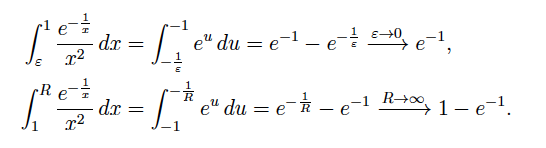
\includegraphics[width=230pt]{images/beispiel_uneigInteg}  \\
			$\Rightarrow$ Unteigentliche Integral konvergent mit $e^{-1} + 1 - e^{-1} = 1	$
	\end{enumerate}
		
	\columnbreak
		% ---
	% Integraltabelle
	\subsubsection*{Integraltabelle ($\rightarrow$ Komplette im Appendix)}




%----------------------------------------------------------
\pagebreak
\subsection*{Differentialrechnung im $\mathbb{R}^n$}

	
	% ------------
	% Differenzierbarkeit
	\subsubsection*{Differenzierbarkeit}
	
	\underline{Partielle Differenzierbarkeit} \\
	$f: \Omega \subset \mathbb{R}^n \to \mathbb{R}^m$ heisst an der Stelle $x_0 \in \Omega$ in Richtung $e_i$ partiell differenzierbar, falls:
	\[
			\lim_{h \to 0} \frac{f(x_0 + he_i)-f(x_0)}{h} =: \frac{\partial f}{\partial x_i} (x_0)
	\]
	existiert.
	\vspace{4mm}
		
	
	\underline{Totale Differenzierbarkeit} \\
	 $f: \Omega \subset \mathbb{R}^n \to \mathbb{R}^m$ heisst an der Stelle $x_0 \in \Omega$ differenzierbar, falls eine lineare Abbildung $A: \mathbb{R}^n \to \mathbb{R}$ existiert mit:
	\[ 
		\lim_{\substack{x \to x_0\\ x \neq x_0}} \frac{f(x)-f(x_0)-A(x-x_0)}{|x-x_0|} =0
	 \]
	Hier ist $df(x_0) = A$  das Differential von $f$ (Jaccobi-Matrix) an der Stelle $x_0$.
	
	% ------------
	% Klasse C^m
	\subsubsection*{Klasse $C^m$}
		$f:\Omega \to \mathbb{R}$ heisst von der Klasse $C^1$, $f \in C^1(\Omega)$, falls $f$ an jeder Stelle $x_0 \in \Omega$ in jede Richting $e_i$ partiell
	differenzierbar ist und falls jede partielle Ableitung stetig ist.
	Die Funktion $f$ heisst weiter von der Klasse $C^m$, falls $ \frac{\partial f}{\partial x^i} \in C^{m-1}(\Omega)_{1 \leq i \leq n} $.

	
	% ------------
	% Partielle Ableitungen
	\subsubsection*{Partielle Ableitungen}
	
	\[
	   \frac{\partial f}{\partial x_i} (x_0) \quad \text{Partielle Ableitung von f nach $x_i$}
	 \]
	 $\Rightarrow $ Alle Variablen ausser $x_i$ werden als Konstante betrachtet.
	
	% ------------
	% Richtungsableitung
	\subsubsection*{Richtungsableitung}
	\[
			D_vf(x,y) = \lim_{h \to 0} \frac{f(x+hv_1 , y+hv_2)-f(x,y)}{h} = df(x,y) \cdot v \quad 
	\]
	
	$\Rightarrow$ Richtungsvektor $v$ nur auf $|v|$ normieren falls nach der Steigung gefragt wird! \vspace{2mm}\\
	
	\underline{Bsp:}		\quad $f(x,y) = (x-2y)^3, \quad p_0=(6,2), \quad v= \begin{pmatrix} 2 \\  1 \end{pmatrix}$ \vspace{1mm}\\
	$df(x,y) = (3(x-2y)^2 , -2 \cdot 3 (x-2y)^2$ \vspace{1mm}\\
	$D_vf(p_0) = df(p_0) \cdot v = (12 , -24) \cdot \begin{pmatrix} 2 \\  1 \end{pmatrix} = 24 - 24 = 0 $ 
	
	
	
	\columnbreak
	% ------------
	% Gradient
	\subsubsection*{Gradient}
		\begin{equation*}
				\text{grad}(f)=\nabla f=
				\begin{pmatrix}
						\frac{\partial f}{\partial x_1}\\
						...\\
						\frac{\partial f}{\partial x_n}\\
				\end{pmatrix}
				 = df^T
		\end{equation*}
		$\Rightarrow$ Zeigt in Richtung des st{\"a}rksten Anstiegs
	
	
	% ------------
	% Hesse-Matrix
	\subsubsection*{Hesse-Matrix}
		Matrix mit allen zweifachen partiellen Ableitungen der Funktion $f: \Omega \rightarrow \mathbb{R}$ 
		\begin{equation*}
			\text{Hess}(f)=
				\begin{pmatrix}
					\frac{\partial^2 f}{\partial^2x_1^2} & ... & \frac{\partial^2 f}{\partial x_1 \partial x_n}\\
					...&...&...\\
					\frac{\partial^2 f}{\partial x_n \partial x_1} & ... & \frac{\partial^2 f}{\partial x_n^2}
				\end{pmatrix}
		\end{equation*}
		
	Identische gemischte Ableitungen $\frac{\partial^2}{\partial x_j \partial x_i}f$	 und $\frac{\partial^2}{\partial x_i \partial x_j}f$\\
	$\Rightarrow $ Hesse-Matrix symmetrisch
	\vspace{5mm}
	
	% ------------
	% Satz von Schwarz
	\subsubsection*{Satz von Schwarz (Kommutativit{\"a}t 2ter Ableit.)}
	Sei $f \in C^2(\Omega)$. Dann gilt:
	\[
			\frac{\partial^2f}{\partial x_i \partial x_j} = \frac{\partial^2f}{\partial x_j \partial x_i} \qquad \forall i,j \in {1, ..., n}
	\]
	 \vspace{2mm}\\
	\underline{Allgemein:} Ist $f: \Omega \rightarrow \mathbb{R}$ auf $\Omega$ m-mal partiell diff'bar und sind alle m-ten Ableitungen in $\Omega$ stetig $\Rightarrow$ Reihenfolge der Differentation spielt bei allen partiellen Ableitungen der Ordnung $\leq$m keine Rolle!
	\vspace{4mm}
	
	
	% ------------
	% Vektorwertige Funktionen & Jaccobi-Matrix
	\subsubsection*{Vektorwertige Funktionen}
		
		\underline{Vekorwertige Funktionen}
		\begin{equation*}
				f: \Omega \subset \mathbb{R}^n \to \mathbb{R}^m, \quad f(x_1, ..., x_n) \to 
					\begin{pmatrix}
						f_1(x_1, ..., x_n) \\
						\vdots \\
						f_m(x_1, ..., x_n)
																			
					\end{pmatrix}
		\end{equation*}
		
		\underline{Differenzial / Jaccobi-Matrix}
		\begin{equation*}
				df = 
					\begin{pmatrix}
						\frac{\partial f_1}{\partial x_1} & ... & \frac{\partial f_1}{\partial x_n} \\
						... & ... & ... \\
						\frac{\partial f_m}{\partial x_1} & ... & \frac{\partial f_m}{\partial x_n}
					\end{pmatrix}
		\end{equation*}
		$\rightarrow$ enth{\"a}lt die $n$ part. Ableit. aller m Komponenten von $f$
	
	
	% ------------
	% Ableitungsregeln
	\subsubsection*{Ableitungsregeln}
		\underline{- Kettenregel} \\
		\[ d\left(f \circ g\right)(x_o) = df\left(g(x_0)\right) dg(x_0) \quad \text{wobei: }f \circ g  = f(g(x))\]
		
		Bsp: \quad $ f(x,y)=\begin{pmatrix} e^x \\ xy \end{pmatrix} \qquad g(x,y,z) = \begin{pmatrix}xy\\y+z\end{pmatrix} $ \\
		\[
				df(x,y)=\begin{pmatrix} e^x & 0 \\ y & x\end{pmatrix} \qquad
				 dg(x,y,z)=\begin{pmatrix} y & x & 0 \\ 0 & 1 & 1 \end{pmatrix}  
		\]
		\[
				df(g(x,y,z)) = \begin{pmatrix} e^{xy} & 0 \\ y+z & xy\end{pmatrix}
		\]
		\[
				df(g(x,y,z)) \cdot dg(x,y,z)= \begin{pmatrix} e^{xy} & 0 \\ y+z & xy\end{pmatrix} \cdot \begin{pmatrix} y & x & 0 \\ 0 & 1 & 1 \end{pmatrix}  
		\]
		\[
				= \begin{pmatrix} ye^{xy} & xe^{xy} & 0 \\ y^2 + yz & 2xy + xz & xy \end{pmatrix}
		\]
		
		\underline{- Umkehrsatz} \vspace{1mm}\\
		Ist $det(df(x_0)) \not = 0$, so ist f lokal umkehrbar. 
		
		\[
				d(f^{-1})(y) = (df(x))^{-1} = \text{Inverse der Jaccobi-Matrix von f}
		\]		

	
	% ------------
	% Taylor mit mehreren Variablen
	\subsubsection*{Taylorentwicklung mit mehreren Variabeln}
	- Formel mit mehreren Variablen \\
	- Beispiel für 3te Ordnung
	 
	
	\pagebreak
	% ------------
	% Kritische / Reguläre Punkte
	\subsubsection*{Kritische / Regul{\"a}re Punkte}
	\begin{itemize}[itemsep=3pt, parsep=2pt, leftmargin=*,align=left]
		\item Fall $f: \mathbb{R}^n \to \mathbb{R} $   \\
				Kriterium : $df(p_0)=0 \rightarrow$ Kritischer Punkt	
					                                                                                                                                                                                                                      
		\item Fall $f: \mathbb{R}^n \to \mathbb{R}^m $ \\
			Kriterium: Rang ($df(p_0)$) nicht max. $\rightarrow$ Kritischer Punkt\\
			 ($Rang(df(p_0)) \leq min\{m,n\}$)
	\end{itemize}
	
	$\Rightarrow $ Nicht kritische Punkte = Regul{\"a}re Punkte \\
	
	Bei Funktionen mit mehreren Variablen werden alle partiellen Ableitungen $= 0$ gesetzt!
	
	% ------------
	% Extremwertaufgaben
	\subsubsection*{Extremwertaufgaben in mehreren Dim.}
	\underline{(1) Notwendige Bedingung:} \vspace{1mm}\\
	Ist $x_0 \in \Omega$ ein lokaler Extremalpunkt (Max., Min.) von f, so gilt: \\
	\[
		df(x_0)=0 \text{d.h. $x_0$ ist ein kritischer Punkt}
	\]
	$\rightarrow$ Kritische Punkte sind Kandidaten f{\"u}r Extremalstellen\\
	 Sattelpunkte (keine Extrema) sind jedoch auch kritische Punkte.
	
	% --
	\vspace{3mm}
	\underline{(2) Kandidaten-Unterscheidung:} 
	\begin{itemize}[itemsep=2pt, parsep=2pt]
		\item $Hess(f)(x_0)$ positiv definit $\Rightarrow$ $x_0$	lokales Min. von f
		\item $Hess(f)(x_0)$ negativ definit  $\Rightarrow$ $x_0$ lokales Max. von f
		\item $Hess(f)(x_0)$ indefinit $\Rightarrow$ $x_0$	Sattelpunkt von  f
		\item $ det(Hess(f)(x_0))=0 $ $\Rightarrow$ Entartung 
	\end{itemize}
	
	\vspace{-2mm}
  	\noindent\textcolor{gray}{\rule{9cm}{0.1pt}}
	\vspace{-2mm}\\
	
	% --
	- Eigenwerte: 
	\begin{enumerate}[label=(\roman*), itemsep=2pt, parsep=2pt]
		\item 	Diagonale der Hesse-Matrix parametrisieren mit (- $\lambda$)
		\item 	Determinate = 0 setzen und $\lambda$'s ermitteln 

	\end{enumerate}

	
	% --
	- Definitheit: 
	\begin{itemize}[itemsep=2pt, parsep=2pt]
			\item positiv definit:	  nur positive Eigenwerte
			\item negativ definit:   nur negative Eigenwerte
			\item indefinit:	 sowohl positive als auch negative. Eigenwerte
	\end{itemize}


	\vspace{2mm}
	% --
	- Hesse-Matrix:
	\vspace{2mm}
	\begin{equation*}
			\text{Hess}(f)=
				\begin{pmatrix}
					\frac{\partial^2 f}{\partial^2x_1^2} & ... & \frac{\partial^2 f}{\partial x_1 \partial x_n}\\
					...&...&...\\
					\frac{\partial^2 f}{\partial x_n \partial x_1} & ... & \frac{\partial^2 f}{\partial x_n^2}
				\end{pmatrix}
		\end{equation*}

		
	\columnbreak		
	% ------------
	% Extremwertaufgaben mit Nebenbedingung
	\subsubsection*{Extremwertaufgaben mit Nebenbedingungen}	
	
	Gegeben: Fkt $f$ und Nebenbedingung-Fkt $g$, ... \\
	Gesucht: Extremum der Fkt. $f$ unter NB $g=0$
	
		\begin{enumerate}[label=(\roman*), itemsep=2pt, parsep=2pt]
			\item Linie ($=$) oder Fl{\"a}che ($\leq$, $<$, $>$, $\geq$)	
			\item NB umschreiben zu: $g=0$
			\item Kandidaten ermitteln
						\begin{enumerate}[ itemsep=2pt, parsep=2pt]
							\item \underline{Linie} \\
									\vspace{-3mm}
									\begin{itemize}
											\item 	Nicht regul{\"a}re Punkte mit $dg=0$ \\
														$\rightarrow$ Testen ob NB auch erf{\"u}llt wird
											\item 	Regul{\"a}re Punkte mit $dL=0$ (Lagrange)
									\end{itemize}
									\vspace{1mm}
							\item \underline{Fl{\"ache}}\\
									\vspace{-3mm}
									\begin{itemize}
											\item 	Kritische Punkte innerhalb mit $df=0$ \\
														$\rightarrow$ Pr{\"u}fen ob innerhalb Fl{\"a}che
											\item 	Rand untersuchen mit Langrange \\
														\vspace{-3mm}
														\begin{itemize}
																\item Falls einfacher Rand: \\
																		- Verfahren wie bei einer Linie anwenden
																\item Falls komplizierter Rand: \\
																		(a) Rand st{\"u}ckweise parametrisieren \\
																		$\rightarrow$ Kritische Punkte der St{\"u}cke ermitteln \\
																		(b) Eckpunkte
														\end{itemize}
									\end{itemize}	
						\end{enumerate}	
			\item 	Typen der Kandidaten ermitteln \\
						$\rightarrow $ Meistens durch Einsetzen in Fkt. \\
						oder ansonsten Hesse-Matrix
		\end{enumerate}

	\vspace{-2mm}
  	\noindent\textcolor{gray}{\rule{9cm}{0.1pt}}
	\vspace{-2mm}\\

	\underline{- Langrange Multiplikatoren Regel} \vspace{1mm}\\
	$x_0$ ist ein kritischer Punkt falls ein $\lambda$ exisitert, s.d. $dL(x_0)=0$
			\[
					\text{Lagrange-Funktion: }L = f - \lambda \cdot g
			\]
			\[
					\text{Kritische Punkte von L falls: } dL(x_0) = 0
			\]
			
	\vspace{1mm}		
	\underline{- Lagrange mit mehreren NB's} \vspace{1mm}\\
			\[
					\text{Lagrange-Funktion: }L = f - \lambda \cdot g_1 - \mu \cdot g_2
			\]
			\vspace{1mm}
			
			\underline{- Verfahren zur Ermittlung:} \vspace{1mm}\\
			- Fkt. L partiell ableiten nach $x_1$, ..., $x_n$ \\
			- Gleichungssystem l{\"o}sen \\
			-- $\lambda$'s gleichsetzen und NB verwenden (evtl. Fallunterscheid.) \\
			-- Gleichungen in einander einsetzen \\
			$\Rightarrow$ Keine L{\"o}sungen vergessen!!

	
	
	\columnbreak
	% ---
	\underline{Rand-Parametrisierung - Beispiel:}
	\begin{itemize}[leftmargin=*,align=left]
			\item 	Auf dem Viereck $ D = \{(x,y) \in \mathbb{R}^2| 0 \leq x \leq 2, 0 \leq y \leq 2 \}$	\\
						mit $f(x,y) = x^2 + 2xy - 4x - 2y$\vspace{1mm}\\
						$\rightarrow$ Unterteilung in 4 Teilst{\"u}cke \\
						(1) $f(0,y) = -2y \rightarrow \frac{df}{dy}=-2 \not = 0$ \\
						(2) $f(2,y) = 4 + 4y -4 -2y \rightarrow \frac{df}{dy}=2 \not = 0$ \\
						(3) $f(x,0) = x^2 -4x \rightarrow \frac{df}{dx}=2x -4 = 0 \Rightarrow x=2$\\
						(4) $f(x,2) = x^2 + 4x - 4x -4 \rightarrow \frac{df}{dx}=2x = 0 \Rightarrow x= 0$\\
						+ Eckpunkte (+ evtl. weiteren Kandidaten)
	\end{itemize}
	
	% ---
	\underline{Viel verwendete NB's: (mit Ursprung 0)}
	\begin{itemize}[ itemsep=2pt, parsep=2pt]
		\item 	Kugeloberfl{\"a}che   \\
					$g(x,y,z) = x^2 + y^2 + z^2 - radius^2 =0$  		
		\item 	Kugelinhalt \\
					$g(x,y,z) = x^2 + y^2 + z^2 \leq radius^2 $ \\
					Rand + Inneres analysieren
		\item 	Kreis \\
					$g(x,y) = x^2 + y^2 - radius^2 = 0$  
		\item 	Kreisfl{\"a}che \\
					$g(x,y) = x^2 + y^2 \leq radius^2$ 
	\end{itemize}
	
	% ---
	\underline{Min./Max. Abstand - Beispiel / Trick} \vspace{1mm}\\
	Abstandsfunktion von Punkt P: \vspace{1mm}\\
	$f(x,y,z) = {\left(\sqrt{(x-P_x)^2 + (y-P_y)^2 + (z-P_z)^2}\right)}^2$ \vspace{2mm}\\
	Nun kann diese Fkt. unter der NB (Bsp.: Gleichung eines K{\"o}rpers) minimiert(max.) werden mit Lagrange \\
	$\rightarrow$ Schlussendlich $\sqrt{\quad}$ ziehen nicht vergessen!

	
	\subsubsection*{Tangentialebene bestimmen}
		\begin{tabular}{lll}
		Gegeben: 		&	Funktion $f(x,y) = ....$ \\
							&	Fl{\"a}che S $:= \{ (x,y,z)  \in \mathbb{R}^3 | z=f(x,y) \}$ \\
							&  Punkt Q $:= (x, y, f(x,y))$ \vspace{1mm}\\
		Gesucht:		& Tangentialebene an S in Punkt Q \\
							& $\Sigma = \{  (x,y,z) \in \mathbb{R}^3 | z = ... \}$ \vspace{1mm}\\
		Verfahren: 	& Falls $f(Q_x,Q_y)$ kritischer Punkt der Fkt. $f$ \\
							& $\Rightarrow$ Tangentialebene konstant mit: \\
							& $\Sigma = \{  (x,y,z) \in \mathbb{R}^3 | z = f(Q_x,Q_y) \}$ \vspace{3mm}\\
		Allg. Formel: & $z = f(Q_x,Q_y) + \frac{\partial f}{\partial x} (x - Q_x) + \frac{\partial f}{\partial y} (y - 					Q_y) $ \\				 
		\end{tabular}
	
	
	
	\subsubsection*{Implizite Funktionen}
		Ziel: Aufl{\"o}sung des Gleichungsystems $f(x,y) = 0$ nach x oder y \\
		
		Der Satz ueber implizite Funktionen gibt Aussagen darueber, ob und unter welchen Bedingungen eine solche lokale Aufloesung existiert oder nicht
		
		
		Untermatrix M des Differentials Invertierbar (det $\not = 0$)  $\Rightarrow $ so ist $f(x,y)$ nach x oder y (je nach Untermatrix M) aufl{\"o}sbar (Zeichnung und Beispiel ergaenzen) \\
		
		
		
		Beispiel: Kann man $f(x,y) = 0$ in der N{\"a}he von $(x,y)=(1,1)$ nach y aufl{\"o}sen? \\
		$\Rightarrow $ Es ist implizt m{\"o}glich, ohne $f$ explizit zu kennen \\
		
		
		
		Falls wir nach x,y aufloesen wollen, muessen wir die partiellen Ableitungen nach x und y betrachten
		
		Ableitung Bestimmbar (Formel)
		\[
				\phi ' = -(M)^{-1} \cdot (Rest der Matrix)
		\]

		Beispiel mit Aufloesung nach x und z (Seite 134)

			
		Beispiele: \\
		$f(x,y) = 2x^2 - 4xy + y^2 -3x + 4y = 0$ \\
		Nach $y$ aufloesen \qquad $y = \phi(x)$ mit $\phi(1)=1$ \\
		\\
		$f(x,\phi(x))=0$
		
		
		BESSER FORMULIEREN (KLARER) +
		LOESUNGSSATZ dazuschreiben (Es existiert eine Umgebung mit blabla)


%----------------------------------------------------------
\pagebreak
\subsection*{Integration im $\mathbb{R}^n$}

	Uebersicht der Verfahren \\
	- Linien-Integrale (Wegintegrale, Potentialfelder, Green)
	+ Umwandlung in Polarkoordinaten \\

	

	% --
	%Vektorfelder, 1Formen - Potentiale
	\subsubsection*{Vektorfelder, 1-Formen und Potentiale}

	\underline{Vekorfeld:} \\
		Funktion die jedem Punkt eines Raumes einen Vektor zuordnet 
		\[
				\vec{v} = \begin{pmatrix} v_1 \\ \vdots \\ v_n\end{pmatrix} 
		\]
		
		\underline{1-Form $\lambda$: }  \quad ( $\lambda = v^T$ ) \\
		
		Bsp: \quad $v_1 dx + v_2 dy + v_3 dz$ \vspace{2mm}\\

		\underline{Rotation:}
		\[
				rot(\vec{v}) = \nabla \times \vec{v} = 
				\begin{pmatrix} 
					\frac{\partial v_3}{\partial y} - \frac{\partial v_2}{\partial z} \\
					\frac{\partial v_1}{\partial z} - \frac{\partial v_3}{\partial x} \\
					\frac{\partial v_2}{\partial x} - \frac{\partial v_1}{\partial y} 
				\end{pmatrix}
		\]
		\underline{Divergenz:}
		
		\[
				div(\vec{v}) = \frac{\partial v_1}{\partial x} + \frac{\partial v_2}{\partial y} + \frac{\partial v_3}{\partial z}
		\]
		
	

	Konservative Vektorfelder \\
	
	-- Potential ermitteln

	\columnbreak
	% ----------------------------
	% Linien-Integrale
	\subsection*{Linien-Integrale}
	
	% --
	% Wegintegrale
	\subsubsection*{- Wegintegral /Potentialmethode}
	
		- Vektorfeld $\vec{v}$ ist meistens gegeben \\
		(manchmal auch als 1-Form $\lambda$  wobei $\lambda = v^T$ )
		
		\begin{enumerate}
			\item 	(Pr{\"u}fen ob ein Potential existiert $\rightarrow$ Vereinfachung) \\
						- Falls ja $\rightarrow $ Weiter mit Punkt 5
			\item	Parametrisierung der Kurve $\gamma$ \\
						\[
						\vec{\gamma} : [a,b] \rightarrow \mathbb{R}^n, t \rightarrow \gamma(t)
						\]
			\item 	Berechne $\dot{\vec{\gamma}}(t) = \frac{d}{dt}\vec{\gamma}(t)$ (jede Komp. nach 		t ableiten)
			\item 	Formel benutzen (Aufpassen: Skalarprodukt)	\\
						\[
							\int_{\gamma} \vec{v} \cdot d\vec{s} = \int_{a}^{b} \langle\vec{v}(\vec{\gamma}(t)) \cdot \dot{\vec{\gamma}}(t)\rangle dt 
						\]
			
			- - - - - - - - - - - - - - - - - - - - - - - - - - - - - - - - - 
			\item 	Falls ein Potential mit $V = \nabla f$ existiert:\\
						\[
							\int_{\gamma} \vec{v} \cdot d\vec{s} = f(\gamma(Ende)) - f(\gamma(Anfang)) 		
						\]
		
		\end{enumerate}


		\vspace{2mm} 
		
		% --
		% Satz von Green 
		\subsubsection*{- Satz von Green (Linienintegrale)}
		siehe Aufgabe 13.3 (Aufpassen auf Richtung)
		
		
		\subsubsection*{- Wichtige Parametrisierungen:}
		Siehe ZF VT \\
		- Parabel
		- Einheitskreis
		- Viertelkreis
		- Ellipse
		- ...
		+ Tipps für gerade Strecke (Muster)
		
		
		\columnbreak
		% -------------------------------------
		% Flächenintegrale
		\subsection*{Fl{\"a}chen-Integrale}
		
		% --
		% Normalbereich
		\subsubsection*{- Integration auf Normalbereichen:}
		Sei
		\[
				\Omega = \{	(x,y) \in \mathbb{R}^2 | a \leq x \leq b, f(x) \leq y \leq g(x)	\}
		\]
		mit stetigen Funktion $f,g$, und sei $F \in C^0$. Dann gilt:
		\[
				\int_{\Omega} F d\mu = \int_{a}^{b} \int_{f(x)}^{g(x)} F(x,y) dy dx
		\]
		
		Beispiel: mit Menge als Normalbereich schreiben + Tipps für Betraege
		
		
		% --
		% Green
		\subsubsection*{- Satz von Green (Fl{\"a}chen):}
		
		\begin{enumerate}
				\item 	Rand parametrisieren
							\[
								\vec{\gamma} : [a,b] \rightarrow \mathbb{R}^n, t \rightarrow \gamma(t)
							\]
				\item 	Berechne $\dot{\gamma}$(Jede Komponente nach t ableiten)
				\item 	$\vec{v}$ w{\"a}hlen (beide haben $rot(\vec{v})=1$):
							\[
										\vec{v} = \begin{pmatrix}0\\x\end{pmatrix}	\quad oder \quad \vec{v} = \begin{pmatrix}-y \\0\end{pmatrix}	
							\]
				\item 	Formel anwenden:
							\[
							   \mu(C) \int_{\gamma = \partial C} \vec{v} \cdot d\vec{s}  \qquad \text{falls: } rot(\vec{v})=1
							\]
							\[
								= \int_{a}^{b} \langle\vec{v}(\vec{\gamma}(t)) \cdot \dot{\vec{\gamma}}(t)\rangle dt 
							\]
		\end{enumerate}

		
		% --
		% Fubini  
		\subsubsection*{- Satz von Fubini / Iterierte Integrale (Quadern):}		
		\[
				\int_{[a,b]\times[c,d]} f(x,y) d\mu(x,y) = \int_{a}^{b} \int_{c}^{d} f(x,y) dy  dx
		\]
		
		$\Rightarrow $ Auf Grenzen aufpassen (Aufabe 12.2)
		
		
		\vspace{-2mm}
  		\noindent\textcolor{gray}{\rule{9cm}{0.1pt}}
		\vspace{-2mm}\\
		
		% -------------------------------------
		% Flussintegrale
		\subsection*{Fluss(Oberfl{\"a}che)-Integrale}
		
		% --
		% Normale Flussintegrale
		\subsubsection*{- Normale Flussintegrale (EVTL LOESCHEN)}

		\begin{enumerate}
			\item Fl{\"a}che S parametrisieren, d.h. finde:
						\[
								\Phi: [a,b] \times [c,d] \rightarrow \mathbb{R}^3, 
						\]
						\[
								(u,v) \rightarrow \Phi(u,v) = (\Phi_1(u,v), \Phi_2(u,v), \Phi_3(u,v))
						\]
			\item Berechne $\Phi_u = \frac{\partial \Phi}{\partial u}$ und $\Phi_v = \frac{\partial \Phi}{\partial v}$
			\item Kreuzprodukt $\Phi_u \times \Phi_v$ berechnen
			\item Formel benutze:
						\[
								\int_{S} \vec{v} \cdot \vec{n}do = \pm \int_{a}^{b} \int_{c}^{d} \langle\vec{v}(\Phi(u,v)) \cdot (\Phi_u \times \Phi_v)\rangle dudv
						\]
		\end{enumerate}



		% --
		% Normale Flussintegrale
		\subsubsection*{- Satz von Gauss}
		\[
				\int_{\partial V} \vec{v} \cdot \vec{n}do = \int_{V} div(\vec{v}) d\mu
		\]
		wobei:
		\[
				div(\vec{v}) = \frac{\partial v_1}{\partial x} + \frac{\partial v_2}{\partial y} + \frac{\partial v_3}{\partial z}
		\]
		
		Beispiel mit Kugelkoordinaten und normales
		Beispiel mit Fluss durch Mantel, Wegnahme von Deckel und Boden

	
		\vspace{-2mm}
  		\noindent\textcolor{gray}{\rule{9cm}{0.1pt}}
		\vspace{-2mm}\\	
		
	\subsubsection*{Transformationssatz}
	\subsubsection*{Substitutionsregel}


		% --
		% Stokes 
		\subsubsection*{- Satz von Stokes}
		Erlaubt es Flussintegrale mithilfe von Wegintegralen zu berechnen.
		
	
	
	Oft vorkommende Integrale
	Wichtige Koordinatentransformationen 13.3 (Seite 218)
	

1-Formen











%----------------------------------------------------------
\pagebreak
\subsection*{Wichtige Verfahren / Grundlagen / Einsortieren}
\subsubsection*{Partialbruchzerlegung (PBZ)}
- Nenner in Linear-Faktoren zerlegen (Faktorisieren $\rightarrow$ nicht 2 identische Faktoren (siehe 2. Beispiel) \\
- Gleichung aufstellen mit $\frac{A}{...}$ + $\frac{B}{...}$ + ... \\
- Gleichnahmig machen \\
- Koeffizientenverglich mittels Matrix (Gauss anwenden) \\

Zum Ansatz werden jeweils abhängig von der Art der Nullstellen folgende Summanden hinzugefügt:
			\begin{enumerate}
				\item einfache Nullstelle $x_i: \quad \frac{a_{i1}}{x-x_i}$
				\item $j$-fache Nullstelle $x_i: \quad \frac{a_{i1}}{x-x_i} + \cdots + \frac{a_{ij}}{(x-x_i)^j} $
				\item
				komplexe Nullstellenpaare: $ \frac{b_ix + c_i}{x^2+p_ix+q_i}$ mit $x^2+p_ix+q_i = (x-z_i)(x- \overline{z_i})$
				wobei das Nennerpolynom die beiden Nullstellen $z_i, \overline{z_i}$ hat.
			\end{enumerate}



Beispiel 1 und Beispiel 2 




\end{multicols*}
\end{document}